% \PassOptionsToPackage{dvipsnames}{xcolor}

% \documentclass[12pt]{spieman}
% % \documentclass[ACS,STIX1COL]{WileyNJD-v2}
% \usepackage{moreverb}
% \usepackage{graphicx} % Required for inserting images
% \usepackage{xcolor}
% % \usepackage{hyperref}
% \definecolor{MyGreen}{RGB}{141,208,138}
% \definecolor{MyBlue}{RGB}{134,190,220}
% \definecolor{MyOrange}{RGB}{252,128,96}
% \definecolor{MyPurple}{RGB}{174,173,211}

% \usepackage{amsmath,amsfonts,amssymb}
% \usepackage{setspace}
% \usepackage{tocloft}
% \usepackage{amsmath}
% \usepackage{multirow}
% \usepackage{placeins}
% \usepackage{subcaption}
% % \captionsetup[figure]{labelfont=normalsize}

% % \articletype{article}

% \newcommand{\figref}[1]{\figurename~\ref{#1}}
% \newcommand{\tabref}[1]{\tablename~\ref{#1}}
% \newcommand{\secref}[1]{Section~\ref{#1}}

% \graphicspath{ {./Figures/} }

% \title{%
% %Application
% Evaluation of a two-layer skin tissue model for diffuse reflectance:
% A simulated and experimental data study}
% \author[1,*]{Anisha Bahl}
% \author[1,3]{Jonathan Shapey}
% \author[2]{Mads Bergholt}
% \author[1]{Tom Vercauteren}
% \affil[1]{School of Biomedical Engineering \& Imaging Sciences, King's College London, 1 Lambeth Palace Road, London, United Kingdom}
% \affil[2]{Department of Craniofacial Development and Stem Cell Biology, King's College London, Guy's Tower, Great Maze Pond, London, United Kingdom}
% \affil[3]{King's College Hospital, Denmark Hill, London, United Kingdom}

% \renewcommand{\cftdotsep}{\cftnodots}
% \cftpagenumbersoff{figure}
% \cftpagenumbersoff{table} 

\chapter[Application of a two-layer skin tissue model]{Application of a two-layer skin tissue model to simulated and experimental data}\label{chap:2layer}

\begin{center}
\begin{minipage}[b]{0.9\linewidth}
\small
\textbf{Foreword\,}
This chapter is an \emph{in extenso} reproduction of a manuscript under preparation for submission to Journal of Biomedical Optics. 
\newline
AB has conducted all of the research presented in this chapter under the supervision of JS, MB, and TV. 
\end{minipage}
\end{center}

\minitoc

% \begin{document}
% \maketitle
% %Abstract must be structured and <200 wds
% \abstract{

% \textbf{Significance} 

% % Tissue oxygenation is established as an important tissue parameter, however traditional pulse oximetry measurements have limits when melanin fraction in the epidermis is high. Due to this, alternative measurement techniques are being explored. 
% Tissue oxygenation ($StO_2$) is established as an important tissue parameter, however these measurements are confounded when melanin fraction in the epidermis is high. 

% \textbf{Aim}

% % We evaluate a two layer diffuse reflectance model
% % %(Yudovsky 2009)
% % proposed by Yudovsky et al. against Monte Carlo simulations of biological tissue. %for diffuse reflectance of biological tissue
% % %is fitted and evaluated against Monte Carlo simulations.
% % We also exploit this model to analyse the open access NIST skin reflectance dataset made available by Cooksey et al. 
% We evaluate a two-layer reflectance model proposed by Yudovsky et al. against Monte Carlo simulations of skin. We also use this model to analyse the open access NIST skin reflectance dataset made available by Cooksey et al. 

% \textbf{Approach}

% % Goodness of fit of the predicted reflectance of the two layer model is evaluated using Monte Carlo simulations with known ground truth. These are also used to evaluate the accuracy of parameter extraction from the inverse problem. %The former have known ground truth physiological parameters, whereas the latter does not. For this reason the goodness of fit of the two-layer forwards model and the parameter extraction quality of the inverse problem are evaluated against Monte Carlo simulations. 
% % The quality of oxygen saturation recovery from the inverse problem is also evaluated with Monte Carlo simulations across a range of melanin volume fractions, epidermal thicknesses, and volume fractions of blood. The inverse problem is used to analyse the NIST skin dataset and the physiological parameters extracted from this are compared to other literature analysis. 
% Simulations are used to evaluate the quality of the modelled reflectance and the extracted physiological parameters. $StO_2$ recovery is examined across ranges of the other physiological parameters. The parameters extracted from the NIST dataset are compared to literature values. 

% \textbf{Results}

% % The normalised root mean squared error between each predicted reflectance and the associated Monte Carlo simulated reflectance is calculated and the means found to be 0.167 and 0.0402 for quantitative or relative data respectively showing that fits are improved when data is normalised. The parameter extraction quality for the same data returns 15.3\% and 13.1\% mean absolute percentage errors for quantitative or relative data respectively showing similar overall quality. A failure region is identified where extraction of tissue oxygenation fails. 
% % %which identifies a significant region of failure. 
% % %To quantify the goodness of fit of this two-layer model against simulated reflectance spectra with known ground truth, the normalised root mean squared error is calculated and the mean found to be 0.167 or 0.0402 for quantitative or relative data respectively. When fitted by least squares, the parameter recovery is quantified using linear regression. By focussing on the quality of the oxygen saturation ($StO_2$) recovery, the performance of this model is evaluated across the parameter range and a significant region of failure identified. 
% % This failure region corresponds to circumstances where the epidermal layer has significant thickness and melanin content, while the dermal layer has low fraction of blood meaning that the haemoglobin impact is “masked”. The extraction of parameters from the NIST skin dataset using this model returns values that do not correspond well to literature values suggesting that, perhaps, many of these spectra lie within a failure region. 
% A failure region of the model is identified characterised by a combination of high melanin content and epidermal thickness, and low dermal blood volume fraction meaning that the haemoglobin impact is “masked”. The parameters extracted from NIST data using this model returns values that do not correspond well to literature values suggesting that many of these spectra may lie within the failure region. 

% \textbf{Conclusions}

% % This work evaluates the Yudovsky et al. two layer model against Monte Carlo simulations and experimental data. This shows that in the majority of physiological parameter space this model recovers oxygen saturation well from simulated data, however its use appears limited when applied to the NIST in vivo dataset. 
% % %This suggests that there are circumstances in which this model performs well, however it should be applied with caution due to its clear regions of failure which limit its use.
% This work evaluates a two-layer model against simulations and experimental data. $StO_2$ is recovered well from simulated spectra in the majority of parameter space, however its use appears limited when applied to in vivo data.
% }
% \keywords{Biological models; Oxygen saturation; Monte Carlo simulations}

% {\noindent \footnotesize\textbf{*}Anisha Bahl,  \linkable{anisha.bahl@kcl.ac.uk} }

\section{Introduction}\label{sec:intro2}
The brain has many layered structures, for example the meninges (dura, pia mater, arachnoid) are all thin layer structures which overlay the cortex. As these are often of the scale that can be penetrated by visible light, this structure should be accounted for in an optical model used to analyse visible spectrum HSI data. Since Yudovsky 2009 was shown to be the best performing single layer model in Chapter~\ref{chap:1layer}, the double layer model of the same publication~\citep{Yudovsky2009} (developed primarily to model skin) is investigated. 

Skin is a layered biological tissue structure which is considered a better defined use case with which to evaluate this layered model. Skin reflectance data obtained using a well-characterised spectroscopic set-up is widely available~\citep{Cooksey2017} and is used for this work. 

% Skin tissue oxygenation ($StO_2$) has been suggested to be a useful metric in the diagnosis and management of pressure ulcers \citep{Wong2003, Mishu2014} and radiative dermatitis \citep{Bashkatov2005}, as well as assisting phlebotomy \citep{FouadAref2021}. For these reasons, efforts have been made to non-invasively quantify $StO_2$ using diffuse reflectance spectroscopy. 

% The diffuse reflectance spectrum of biological tissue is influenced by its absorbance and scattering properties.
% %of the tissue.
% Scattering  of tissue is largely dominated by collagen \citep{Anderson1981}. Absorbance of tissue is governed by the chromophores present and is typically dominated by haemoglobin which can exist in both oxygenated and deoxygenated states\citep{Prahlc}.
% These two forms of haemoglobin have differences in absorption which influence the diffuse reflectance spectrum and may allow recovery of the tissue $StO_2$ \citep{Clancy2020}. 

% Many methods have been used to quantify $StO_2$ in vivo \citep{Nitzan2020} with pulse oximetry being the most widely utilised non-invasive method, however these devices have been reported to have different performance quality with respect to different ethnicities \citep{Bangash2022}. More advanced, multi-layered, optical models of tissues have been proposed \citep{Maeda2010}. In this work we focus our analysis in the visible spectrum (450-650nm) as this allows for non-contact imaging using standard cold surgical light sources \citep{Clancy2011}. We investigate one multi-layered, analytical model proposed by Yudovsky et al. \citep{Yudovsky2009} which utilises a single layer model which we have previously shown demonstrates excellent results \citep{Bahl2023a}. The authors show the model to perform poorly above 600nm \citep{Yudovsky2011a} and so we restrict our evaluation range accordingly. 
% % from diffuse reflectance spectroscopy, however few model the spectrum per wavelength, and fewer still provide this modelled spectrum for skin which is characterised by a layered structure. A notable example of this is the Yudovsky 2009 \citep{Yudovsky2009} based on the Kubelka-Munk theory. 
% Whilst this model has been demonstrated with a variety of experimental data \citep{Yudovsky2011a, Yudovsky2011b},
% %there has not been a clear evaluation of its performance. 
% a systematic and reproducible evaluation of its performance is still lacking. 

% % Yudovsky's two-layer model builds on a single-layer model which could also be used to capture average tissue parameters across layers.
% % In this work, we evaluate the two-layer model against the one-layer version
% % %we have also evaluated alongside
% % and also consider
% % two other prominent single-layer tissue models (a modified Beer-Lambert model \citep{Clancy2015}, and a more elaborate Beer-Lambert-based model proposed by Jacques \citep{Jacques1999}).
% % %\citep{Bahl2023a}.
% % These one-layer models are conceptually better suited to open surgical cases where the tissue seen can be approximated as a single homogeneous layer
% % and we refer the reader to our previous work for a head-to-head comparison in the single layer scenario \citep{Bahl2023a}.

Monte Carlo simulations may be used to model
the interaction of light with
both homogeneous and layered tissues
% interactions with light of
over a range of optical wavelengths.
These simulations can be used to predict the diffuse reflectance spectrum of a tissue given known constituents. Whilst Monte Carlo is a well-established simulation approach, it is highly computationally challenging to use this to solve for the corresponding inverse problem. This inverse problem, however, is key to clinical translation where in vivo diffuse reflectance measurements of tissue can be obtained non-invasively, for example using hyperspectral imaging~\citep{Clancy2020}. Solving the inverse problem could allow for these measurements to be used to identify the constituent make-up of the sample being imaged. 

In this chapter, we aim to quantify the performance of the two-layer Yudovsky model by evaluating both the forwards model and inverse problem performance against a Monte Carlo dataset with known ground-truth parameters. The quality of the forwards model is quantified by evaluating the similarity of the predicted diffuse reflectance spectra to Monte Carlo simulated spectra using the same ground truth parameters. The fidelity of the parameter extraction is quantified by comparing the parameters generated by fitting to the Monte Carlo simulated spectra to the ground truth parameters used to generate the simulations.

We also fit the two-layer model to experimental data made available by NIST~\citep{Cooksey2017}, and compare the extracted parameters to literature values. This allows us to evaluate the use of this model to solve the inverse problem.
This leads to a thorough evaluation of the Yudovsky two-layer model and enables informed application to clinical settings. 

\section{Methods}\label{sec:methods2}
% \subsection{Single-layer models}\label{sec:methodtissuemodelsingle}
% Three analytical models are compared in this work: modified Beer-Lambert \citep{Clancy2015}, Jacques 1999 \citep{Jacques1999}, and Yudovsky 2009 \citep{Yudovsky2009}. Each of these provide analytical models aiming to investigate single-layer, homogeneous, semi-infinite tissue to enable analysis of tissue during surgery. All three models contain hyperparameters to account for the impact of changes in refractive index which are fitted Monte Carlo simulations, where a single set of values is fitted to a dataset of 100 spectra using the ground truth tissue parameter values. \textcolor{red}{CITE 1LAYER PAPER}

% \subsubsection{Common absorption and scattering model}\label{sec:opticproperties}
% All three forward models utilise the wavelength dependent absorption and reduced scattering coefficients ($\mu_a(\lambda)$ and $\mu_s'(\lambda)$) to compute a
% diffuse reflectance spectrum. 
% The reduced scattering coefficient relates the scattering coefficient ($\mu_s(\lambda)$) with tissue anisotropy ($g$) as follows: 
% \begin{equation}
%     \mu_s'(\lambda) = \mu_s(\lambda) \times (1-g)
%     \label{eq:reducedscattering}
% \end{equation}
% For biological tissue, the reduced scattering coefficient can be well approximated using Mie theory \citep{Jacques2013}: 
% \begin{equation}
%     \mu_s'(\lambda) = a(\frac{\lambda}{500})^{-b}
%     \label{eq:Mie}
% \end{equation}
% where $a$ and $b$ are Mie scattering coefficients that range between 8\textrm{$cm^{-1}$} and 70\textrm{$cm^{-1}$}, and 0.1 and 3.3 respectively depending on the tissue microstructure \citep{Jacques2013}. 
% The absorption coefficient of most internal, homogeneous, tissues, including dermis, is dominated by haemoglobin in the visible region (450-650 nm)\citep{JacquesAbs} and can be modelled using the following equation \citep{Yudovsky2009}: 
% \begin{equation}
% \begin{aligned}
%     & \mu_a(\lambda) = f_{blood}\mu_{a, blood}(\lambda) + (1 - f_{blood})\mu_{a, back}(\lambda) \\
%     & \textrm{where} \\
%     & \mu_{a, blood}(\lambda) = c_{HbT}\frac{\ln(10)}{64500}[StO_2 \epsilon_{HbO_2}(\lambda) + (1 - StO_2)\epsilon_{Hb}(\lambda)] \\
%     & \textrm{and} \\
%     & \mu_{a, back}(\lambda) = 7.84\times10^8 \lambda^{-3.255}
% \end{aligned}
% \label{eq:mua}
% \end{equation}
% Here $StO_2$ refers to oxygen saturation, $c_{HbT}$ refers to the total concentration of haemoglobin in whole blood commonly taken as 150\textrm{$gL^{-1}$}\citep{Prahlb}, with $StO_2$ denoting the fraction of haemoglobin that is oxygenated ($HbO_2$) and the remainder is deoxygenated ($Hb$), and ranges between 0-100\%\citep{Yudovsky2009}. $f_{blood}$ is the volume fraction of tissue occupied by blood which has absorption coefficient $\mu_{a, blood}(\lambda)$ and typically ranges between 0.2-12\%\citep{Yudovsky2009}, with the remainder of tissue having background absorption $\mu_{a, back}(\lambda)$\citep{Yudovsky2009}.
% Finally, $\epsilon_{HbO_2}(\lambda)$ and $\epsilon_{Hb}(\lambda)$ denotes the wavelength-dependent extinction coefficients of the chromophores $HbO_2$ and $Hb$ which are found in the literature\citep{Prahlb}. 

% \subsubsection{Modified Beer-Lambert}
% The modified Beer-Lambert models absorption ($A(\lambda)$) and diffuse reflectance ($R(\lambda)$) as follows: 
% \begin{equation}
% \begin{aligned}
%     & A(\lambda) = L\mu_a(\lambda) + \mu_s'(\lambda) \\
%     & R(\lambda) = \exp{\left(-\frac{A(\lambda)}{100}\right)}
% \end{aligned}
% \label{eq:modBL1}
% \end{equation}
% A factor of 100 is included to convert $\mu_a(\lambda)$ and $\mu_s'(\lambda)$ from the conventional units of cm\textrm{$^{-1}$} to mm\textrm{$^{-1}$}. $L$ describes a differential path length to account for the variety of photon path lengths through scattering media. To simplify this model, $L$ is often approximated to 1 \citep{Clancy2015} and $\mu_s'(\lambda)$ is often modelled as a wavelength-independent constant\citep{Clancy2015, Ma2016}. 
% To allow for improved flexibility in this model,
% we introduce linear scaling hyperparameters ($M_{1-3}$), as shown in Equation~\eqref{eq:modBL2}, that are fitted to Monte Carlo simulations at the refractive index of interest. 
% \begin{equation}
% \begin{aligned}
%     & A(\lambda) = M_1\mu_a(\lambda) + M_2\mu_s'(\lambda) + M_3 \\
%     & R(\lambda) = \exp{\left(-\frac{A(\lambda)}{100}\right)}
% \end{aligned}
% \label{eq:modBL2}
% \end{equation}

% \subsubsection{Jacques 1999}
% The Jacques model is also based on the Beer-Lambert model using the assumption that a wavlength-dependent path length $L(\lambda)$ can approximate the ensemble of path lengths experienced by photons in a tissue by $L(\lambda) = A(\lambda)\delta(\lambda)$ where $A(\lambda)$ and $\delta(\lambda)$ are defined in Equation~\eqref{eq:Jacques}. This results in the following model with the hyperparameters ($M_{1-3}$) which the authors fit to Adding Doubling simulations \citep{Jacques1999}. In our work, we refit these to Monte Carlo simulations since these are considered the gold standard optical simulation method and improve the model fitting results. 
% \begin{equation}
% \begin{aligned}
%     & N'(\lambda) = \frac{\mu_s'(\lambda)}{\mu_a(\lambda)} \\
%     & \delta(\lambda) = \frac{1}{\sqrt{3\mu_a(\lambda)[\mu_a(\lambda) + \mu_s'(\lambda)]}} \\
%     & A(\lambda) = M_1 + M_2\exp \left[ \frac{\ln(N'(\lambda))}{M_3} \right] \\
%     & R(\lambda) = \exp[-A(\lambda)\delta(\lambda)\mu_a(\lambda)] \\
% \end{aligned}
% \label{eq:Jacques}
% \end{equation}

% \subsubsection{Yudovsky 2009}\label{sec:Yudovskysingle}
% \subsection{Double-layer model}\label{sec:methodtissuemodeldouble}
\subsection{Modelling diffuse reflectance of biological tissues}\label{sec:methodtissuemodeldouble}
Throughout this work we will adopt the convention where the epidermal layer is numbered 1, with deeper layers labelled sequentially. This replicates the naming conventions of Yudovsky et al. in their original publication of this model~\citep{Yudovsky2009}. Here this corresponds to the epidermal layer being denoted 1 and the dermal layer 2. 
%
\subsubsection{Common absorption and scattering model}\label{sec:opticproperties2}
% The Yudovsky 2009 model utilises a wavelength dependent absorption and reduced scattering coefficient for each tissue layer, $\mu_a(\lambda)$ and $\mu_s'(\lambda)$ respectively, to compute a diffuse reflectance spectrum. 
As described in Chapter~\ref{chap:1layer}, the forwards model for each layer utilises the wavelength dependent absorption coefficient $\mu_a(\lambda)$ and reduced scattering coefficient $\mu_s'(\lambda)$ to compute a diffuse reflectance spectrum. The reduced scattering coefficient of both dermis and epidermis is modelled identically to that in Section~\ref{sec:opticproperties}.
% The reduced scattering coefficient relates the scattering coefficient $\mu_s(\lambda)$ with tissue anisotropy $g$ as follows: 
% \begin{equation}
%     \mu_s'(\lambda) = \mu_s(\lambda) \times (1-g)
%     \label{eq:reducedscattering}
% \end{equation}
% For biological tissue, the reduced scattering coefficient can be well approximated using Mie theory \citep{Jacques2013}: 
% \begin{equation}
%     \mu_s'(\lambda) = a(\frac{\lambda}{500})^{-b}
%     \label{eq:Mie}
% \end{equation}
% where $a$ and $b$ are Mie scattering coefficients that range between 8 cm$^{-1}$ and 70 cm$^{-1}$, and 0.1 and 3.3 respectively depending on the tissue microstructure \citep{Jacques2013}. 
Yudovsky et al. specify a single $\mu_s'(\lambda)$ to describe the scattering of both epidermis and dermis. 

The absorption coefficient of most homogeneous tissues can be modelled by the sum of the wavelength-dependent absorption coefficients of each major component multiplied by their volume fractions~\citep{Jacques2013}. 
This can be seen in Equation~\eqref{eq:generalmuaJacques} where $f$ is the volume fraction of each component $i$ with corresponding absorption coefficient $\mu_a(\lambda)$ at each wavelength $\lambda$. 
\begin{equation}
    \mu_a = \sum_i{f_i\mu_{a, i}(\lambda)}
    \label{eq:generalmuaJacques}
\end{equation}
In this work we specify the major components to be blood, melanin, and a background component accounting for all other chromophores whose impact are low in this wavelength range. This is shown in Equation~\eqref{eq:generalmua} where blood, melanin, and background are denoted $blood$, $mel$, and $back$ respectively.
\begin{equation}
    \mu_a = f_{blood}\mu_{a, blood}(\lambda) + f_{mel}\mu_{a, mel}(\lambda) + (1 - f_{blood} - f_{mel})\mu_{a, back}(\lambda)
    \label{eq:generalmua}
\end{equation}
When modelling skin, it is necessary to use more than one layer due to the stark differences in optical and anatomical properties between the layers of skin~\citep{Mignon2018}. The epidermal layer absorption is dominated by the chromophore melanin and is largely devascularised so Equation~\eqref{eq:generalmua} can be simplified to a two-component system as shown in Equation~\eqref{eq:muaepi}~\citep{Yudovsky2009}.
\begin{equation}
\begin{aligned}
    & \mu_{a, 1}(\lambda) = f_{mel}\mu_{a, mel}(\lambda) + (1-f_{mel})\mu_{a, back}(\lambda) \\
    %& \textrm{where}\\
    & \mu_{a, mel}(\lambda) = 6.60\times10^{11}\lambda^{-3.33}\\
    %& \textrm{and}\\
    & \mu_{a, back}(\lambda) = 7.84\times10^8\lambda^{-3.255}\\
\end{aligned}
\label{eq:muaepi}
\end{equation}
The absorption coefficient of most internal, homogeneous, tissues, including dermis as in the Yudovsky 2009 formulation, is dominated by haemoglobin in the visible region, 450-650 nm~\citep{JacquesAbs} and has no contribution from melanin. This allows Equation~\eqref{eq:generalmua} to be simplified to another two-component system as shown in Equation~\eqref{eq:mua2}~\citep{Yudovsky2009} which is identical to that seen in Chapter~\ref{chap:1layer}: 
\begin{equation}
\begin{aligned}
    & \mu_{a, 2}(\lambda) = f_{blood} \mu_{a, blood}(\lambda) + (1 - f_{blood})\mu_{a, back}(\lambda) \\
    %& \textrm{where} \\
    & \mu_{a, blood}(\lambda) = c_{HbT}\frac{\ln(10)}{64500}\large[StO_2 \epsilon_{HbO_2}(\lambda) + (1 - StO_2)\epsilon_{Hb}(\lambda)\large] \\
    %& \textrm{and} \\
    & \mu_{a, back}(\lambda) = 7.84\times10^8 \lambda^{-3.255}
\end{aligned}
\label{eq:mua2}
\end{equation}
Here $StO_2$ refers to oxygen saturation
and ranges between 0-100\%.
$c_{HbT}$ refers to the total concentration of haemoglobin in whole blood commonly taken as 150 gL$^{-1}$~\citep{Prahl1999}.
% %With $StO_2$ denoting the fraction of haemoglobin that is oxygenated, $HbO_2$, and the remainder being deoxygenated, $Hb$,
% %$StO_2$ ranges between 0-100\%\citep{Yudovsky2009}.
% $f_{blood}$ is the volume fraction of tissue occupied by blood which has absorption coefficient $\mu_{a, blood}(\lambda)$ and typically ranges between 0.2-12\%\citep{Yudovsky2009}.
% The remainder of tissue is modelled using a background absorption term $\mu_{a, back}(\lambda)$ which takes account of the impact of other chromophores in bulk tissue \citep{Yudovsky2009}.
Finally, $\epsilon_{HbO_2}(\lambda)$ and $\epsilon_{Hb}(\lambda)$ denotes the wavelength-dependent extinction coefficients of the oxygenated and de-oxygenated haemoglobin chromophores $HbO_2$ and $Hb$ which are found in the literature~\citep{Prahl1999}. 
% Each of these layers has a distinct absorption coefficient $\mu_a(\lambda)$ and identical reduced scattering coefficient $\mu_s'(\lambda)$.
% The epidermal 
% %$\mu_a(\lambda)$ (
% absorption coefficient $\mu_{a, 1}(\lambda)$ is modelled with the major chromophore melanin, characterised by its volume fraction $f_{mel}$ (ranging between 1-43\% \citep{Yudovsky2009}) and no blood, as described
% below:
%in Equation~\eqref{eq:muaepi}. 

The tissue parameters are restricted by Yudovsky to 20-100\% for $StO_2$, 0.2-7\% for $f_{blood}$~\citep{Yudovsky2011a} and we limit the scattering tissue parameters to 30-70cm$^{-1}$ and 0.7-2.5 for $a$ and $b$ respectively to reflect those of skin~\citep{Jacques2013}. 

\subsubsection{Layered model formulation for diffuse reflectance}\label{sec:Yudovsky2009}
% The original Yudovsky model presents a complex analytical derivation \citep{Yudovsky2009} of a single-layer reflectance equation for each tissue layer with a simplified formulation subsequently presented in their Erratum \citep{Yudovsky2015}. The model takes the reduced albedo $w'(\lambda)$, calculated from $\mu_a$ and $\mu_s'$, as input and returns the diffuse reflectance spectra $R(\lambda)$.
% This provides an easily applicable model with hyperparameters $M_{1-6}$ which are quoted for a refractive index $n$ of 1.44. We found that hyperparameters $M_{1-6}$ can be fitted to Monte Carlo spectra to allow for use with other refractive indices \citep{Bahl2023a}. The hyperparameters found by fitting to a Monte Carlo dataset with a refractive index of 1.44 are used throughout this work \citep{Bahl2023a}. This simplified formulation is used within this work:
% \begin{equation}
% \begin{aligned}
%     & w'(\lambda) = \frac{\mu_s'(\lambda)}{\mu_a(\lambda) + \mu_s'(\lambda)} \\
%     & R = M_1 + M_2\exp{\left[ M_3w'(\lambda)^{M_4}\right]} + \frac{M_5}{1.02 - M_6} \\
% \end{aligned}
% \label{eq:Yudovskysingle}
% \end{equation} 
% 
The Yudovsky two-layer model is a complex interaction between two instances of the Yudovsky single-layer model~\citep{Yudovsky2009}, detailed in Section~\ref{sec:Yudovskysingle}, applied to two layers~\citep{Yudovsky2009}. 
These two layers represent the epidermis ($1$) and dermis ($2$), where the former has thickness $L_1$ and the latter is semi-infinite. $L_1$ is input to the model in units of cm, however it is discussed throughout in \textmu m for ease of interpretation.
These single layer reflectances are then combined as in Equation~\eqref{eq:Pilondouble} using a reduced reflectance ($R^*$) which is calculated using $L_1$, $w_{tr, 1}$, and $w_{tr,2}$ as 
%in Equation~\eqref{eq:reducedR}. 
shown below:
\begin{equation}
\begin{aligned}
    & \xi = \sqrt{\frac{47}{52} + \frac{31}{49}w_{tr, 1} - \frac{49}{54}w_{tr, 1}^2 - \frac{17}{27}w_{tr, 1}^3} \\
    & Y_1 = \xi(\mu_{a,1} + \mu_s')L_1 \\
    & \frac{1}{\alpha} = 2.562 - \frac{4.263}{3.050 - w_{tr, 2}} \\
    & R^* = \frac{\tanh{Y_1}}{\frac{1}{\alpha} + (1 - \frac{1}{\alpha})\tanh{Y_1}} \\
\end{aligned}
\label{eq:reducedR}
\end{equation} 
%Equation~\eqref{eq:Pilondouble} returns the diffuse reflectance spectrum, however this can be converted to total reflectance by addition of a constant offset of 0.0325 for a refractive index of 1.44 (for tissues)\citep{Yudovsky2011a}.
\begin{equation}
    R = R^*(R_{s1} - R_{s2}) + R_{s2}
\label{eq:Pilondouble}
\end{equation}
Whilst Equation~\eqref{eq:Pilondouble} returns diffuse reflectance values, Yudovsky et al. present a conversion to total reflectance ($R_{tot}$) values by addition of a wavelength independent specular reflectance ($R_{sp}$) term equalling 0.0325 for a refractive index of 1.44 as seen in Equation~\eqref{eq:Pilontotal}~\citep{Yudovsky2011a}.
\begin{equation}
    R_{tot} = R^*(R_{s1} - R_{s2}) + R_{s2} +R_{sp}
\label{eq:Pilontotal}
\end{equation}

\subsection{Inverse problem fitting to recover tissue parameters}\label{sec:methodinverse}
This formulation for reflectance presented in Section~\ref{sec:Yudovsky2009} ($R$) can be used to solve the inverse problem, shown in Equation~\eqref{eq:inverseproblem}, by fitting to a reflectance spectrum ($R_{ref}$). 
\begin{equation}
    \argmin_{StO_2, f_{blood}, f_{mel}, L_1, a, b} \sum || R_{ref}(\lambda) - R(\lambda) ||^2
    \label{eq:inverseproblem}
\end{equation}
This is fitted using a least squares fitting approach (using SciPy v1.10.0  \newline \href{https://docs.scipy.org/doc/scipy/reference/generated/scipy.optimize.least_squares.html}{\texttt{scipy.optimize.least\_squares}} function) which allows extraction of physiological parameters. 
Yudovsky et al. note that this model is not suitable for wavelengths above 600 nm~\citep{Yudovsky2011a} and therefore only wavelengths below 600nm are considered for this analysis. Similarly, Yudovsky et al. present results using wavelengths above 450 nm so we utilise the same wavelength range. We have found that increasing the weighting in the region 525-585nm, ie. the region corresponding to the major haemoglobin peaks, improves the fit of this model in this region. The weighting function used can be seen in \figref{fig:weighting} and is used throughout this work, however we provide similar analyses of the data with a uniform wavelength weighting in the Appendices Section~\ref{ap:2layeruniform}. 
\begin{figure}
    \centering
    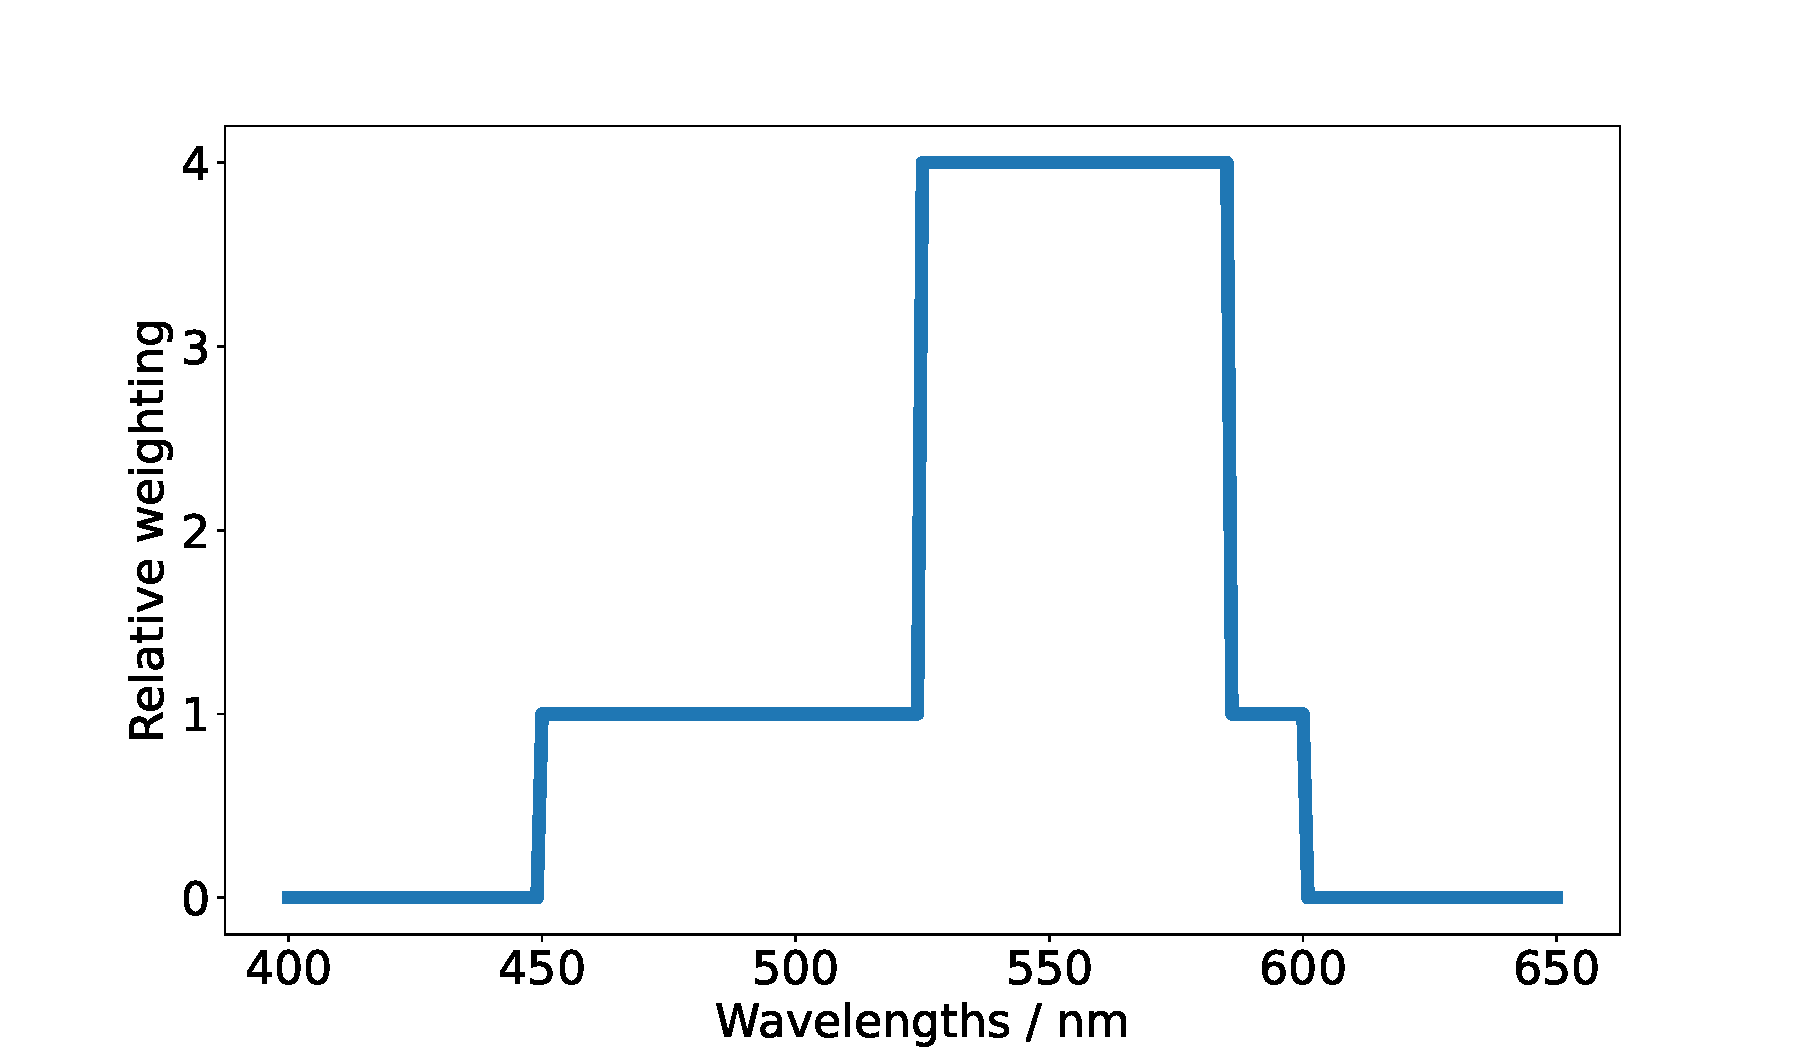
\includegraphics[width=0.6\textwidth]{fitting_region}
    \caption{Relative weighting of wavelengths used for least squares fitting of the two-layer Yudovsky model. The wavelengths considered are limited to 450-600nm to replicate those recommended by Yudovsky et al. An increased weighting is placed on the wavelength range 525-585nm to improve the visual fitting of this region which contains the major haemoglobin peaks.}
    \label{fig:weighting}
\end{figure}
Bounds are also imposed on the least squares fitting routine to ensure the fitted parameters are feasible and within a biologically relevant range for skin~\citep{Yudovsky2009, Jacques2013} such that:
\begin{itemize}
    \item 30cm$^{-1}$ $<=$ $a$ $<=$ 70cm$^{-1}$
    \item 0.7 $<= b <=$ 2.5
    \item 20\% $<= StO_2 <=$ 100\%
    \item 0.2\% $<= f_{blood} <=$ 7\% 
    \item 1\% $<= f_{mel} <=$ 43\% 
    \item 20{\textmu}m $<= L_1 <=$ 150{\textmu}m
\end{itemize}
Often in clinical settings it is difficult to obtain precise quantitative data and so relative data is used instead~\citep{Bahl2023}. For the
purposes of this work, we define relative data to be mean normalised spectra using the mean of all wavelengths in the range 450-600nm which can be applied to both $R$ and the simulated or measured data. 
%
%Often in clinical settings it is difficult to obtain precise quantitative data and so relative data is used instead\citep{Bahl2023}. For the purposes of this work, we define relative data to be mean normalised spectra using the mean of all wavelengths below 600nm. 

\subsection{Reference spectra}\label{sec:methodreference2}
%100
\subsubsection{Simulated dataset}
Similarly to Section~\ref{sec:methodreference}, one hundred
Monte Carlo simulations are generated by selecting random values for the variables $a$, $b$, $StO_2$, $f_{blood}$, $f_{mel}$, and $L_1$ within the bounds detailed in Section~\ref{sec:methodinverse}.
%which are bounded to 30-70 cm$^{-1}$, 0.7-2.5, 20-100\%, 0.2-7\%, 1-43\%, and 20-150 {\textmu}m respectively to represent the range seen in skin \citep{Jacques2013, Yudovsky2009}.
These are converted to $\mu_a$ and $\mu_s'$ values as in \secref{sec:opticproperties2}. Monte Carlo takes $\mu_a$ and $\mu_s$ as inputs for each layer so a random value of $g$ is chosen per spectrum between 0.7-0.9 to convert $\mu_s'$ to $\mu_s$ using Equation~\eqref{eq:reducedscattering}. The diffuse reflectance spectra are then generated using CUDAMCML~\citep{Alerstam2008}, a GPU accelerated adaptation of the MCML programme for MC simulations of layered media with semi-infinite widths~\citep{Wang1995, Prahl1989}, to propagate 10000 photons through a geometry of a slab of thickness $L_1$ of epidermis with optical properties $\mu_{a,1}$ and $\mu_s'$ and a 3cm slab of dermis with optical properties $\mu_{a, 2}$ and $\mu_s'$. This depth is chosen to approximate a semi-infinite depth; for many tissues, the impact of increasing the depth of tissue is negligible beyond depths of 1 cm~\citep{Zhang2014}. When fitting models to these spectra for parameter extraction, the same bounds are imposed on the fitting routine. 

\subsubsection{Measured dataset}
An existing NIST reflectance dataset made available by Cooksey et al.~\citep{Cooksey2017} is chosen to evaluate the model's performance on in vivo skin measurements. This dataset measured total reflectance from the forearms of 100 healthy volunteers using an integrating sphere spectrophotometer~\citep{Cooksey2017}. Three replicates were measured of which we utilise the mean for each volunteer to create the reference set of 100 spectra used for this work. This dataset is one of the few, or only, open access skin reflectance datasets and is chosen due to the high quality spectral measurement using a controlled integrating sphere measurement protocol. There are, however, no associated ground truth composition parameters for the subjects measured in this study. We also normalise this data by the mean of the wavelengths in the region 450-600nm to construct relative measured data for investigation. 
\FloatBarrier

\subsection{Evaluation of model performance}\label{sec:methodevaluate2}
Throughout this chapter the evaluation methods are performed on both quantitative and relative spectra, where the relative spectra are generated by normalisation using the mean taken from the range 450-600nm.
\subsubsection{Simulated dataset}
The forwards model and inverse problem is evaluated against diffuse reflectance spectra generated using Monte Carlo simulations detailed in \secref{sec:methodreference2} in a similar manner to those in Section~\ref{sec:methodevaluate}. 
%%This model is evaluated against reference spectra with known ground truth parameters generated using Monte Carlo as detailed in \secref{sec:methodreference}, and experimental data as provided by a NIST skin dataset\citep{Cooksey2017}, which does not have known ground truth parameters. 
%
% The similarity of each diffuse reflectance spectrum predicted using the forward Yudovsky 2009 model ($s$) and the corresponding spectrum generated using Monte Carlo simulation ($r$) using the same ground truth physiological parameters at all wavelengths ($\lambda$) are quantified using the Normalised Root Mean Squared Error ($NRMSE$):
% %, defined in Equation~\eqref{eq:NRMSE}.
% \begin{equation}
%     NRMSE = \frac{\sqrt{\frac{1}{\Lambda}\sum_{\lambda}^{\Lambda}\left(s_{\lambda} - r_{\lambda}\right)^2}}{\sqrt{\frac{1}{\Lambda}\sum_{\lambda}^{\Lambda} r^2_{\lambda}}}
%     \label{eq:NRMSE}
% \end{equation}

% We investigate the inverse problem by fitting the physiological parameters to simulated diffuse reflectance spectra with known ground truth parameters. 
% %using a least squares approach. 
% The correlation between the ground truth and fitted parameters is calculated (using SciPy v1.10.0 \href{https://docs.scipy.org/doc/scipy/reference/generated/scipy.stats.linregress.html}{\texttt{scipy.stats.linregress}} function) and evaluated using the Pearson correlation coefficient $r$ and the p-value $p$.
% We take $p < 0.05$ to demonstrate significance at a 95\% confidence level for a hypothesis test with the null hypothesis that there is no correlation. 

To demonstrate the regions of parameter space where the Yudovsky two-layer model varies in performance quality, for each combination of absorbance parameters (and one set of scattering parameters) 10 Monte Carlo diffuse reflectance spectra are simulated where the $StO_2$ is varied between 0 and 100\% and scattering parameters are fixed. The Yudovsky two-layer model is fitted to each of these Monte Carlo spectra and a linear regression is fitted between the extracted and input $StO_2$. The $r$ value is then plotted in the remaining 3D parameter space ($f_{blood}$, $f_{mel}$, $L_1$) and coloured by value.

\subsubsection{Measured dataset}
The inverse problem can also be applied to the NIST skin dataset~\citep{Cooksey2017}. The model is fit to the total reflectance spectra in the NIST skin dataset. As there are no ground truth parameters available for this dataset, the recovered parameters from these 100 spectra are simply visualised as box and violin plots to compare to literature values for healthy individuals~\citep{Jacques2013, VanManen2021, Nishidate2011, Lintzeri2022}. \citet{VanManen2021} uses a modified Beer-Lambert-based model to analyse HSI images of skin using spatial regularisation, whereas \citet{Nishidate2011} uses a deep learning model trained using 3-layer Monte Carlo skin difuse reflectance simulations to analyse RGB images of skin. 
%\FloatBarrier

\section{Results}\label{sec:results2}
% \subsection{Double-layer model}\label{sec:results2layer}

\subsection{Simulated data}\label{sec:resultsMC2}
Spectra predicted by the forwards Yudovsky two-layer model are compared to those simulated by Monte Carlo simulated diffuse reflectance spectra. The mean ($\pm$ standard deviation) $NRMSE$ between the two for the same ground truth parameters at wavelengths in the range 450-600nm for a refractive index of 1.44 is 0.167($\pm$ 0.133) for quantitative data and 0.0402 ($\pm$ 0.0289) for relative data demonstrating considerable variability in the quality of fit for quantitative data which is significantly reduced by mean normalisation. This reduction in variability of fit can also be seen in some exemplar spectra shown in \figref{fig:egtwolayerMCforwards} and \figref{fig:egtwolayerMCforwardsnorm} for quantitative and relative data respectively. 
\begin{figure}[htbp]
    \centering
    \begin{subfigure}{0.49\textwidth}
        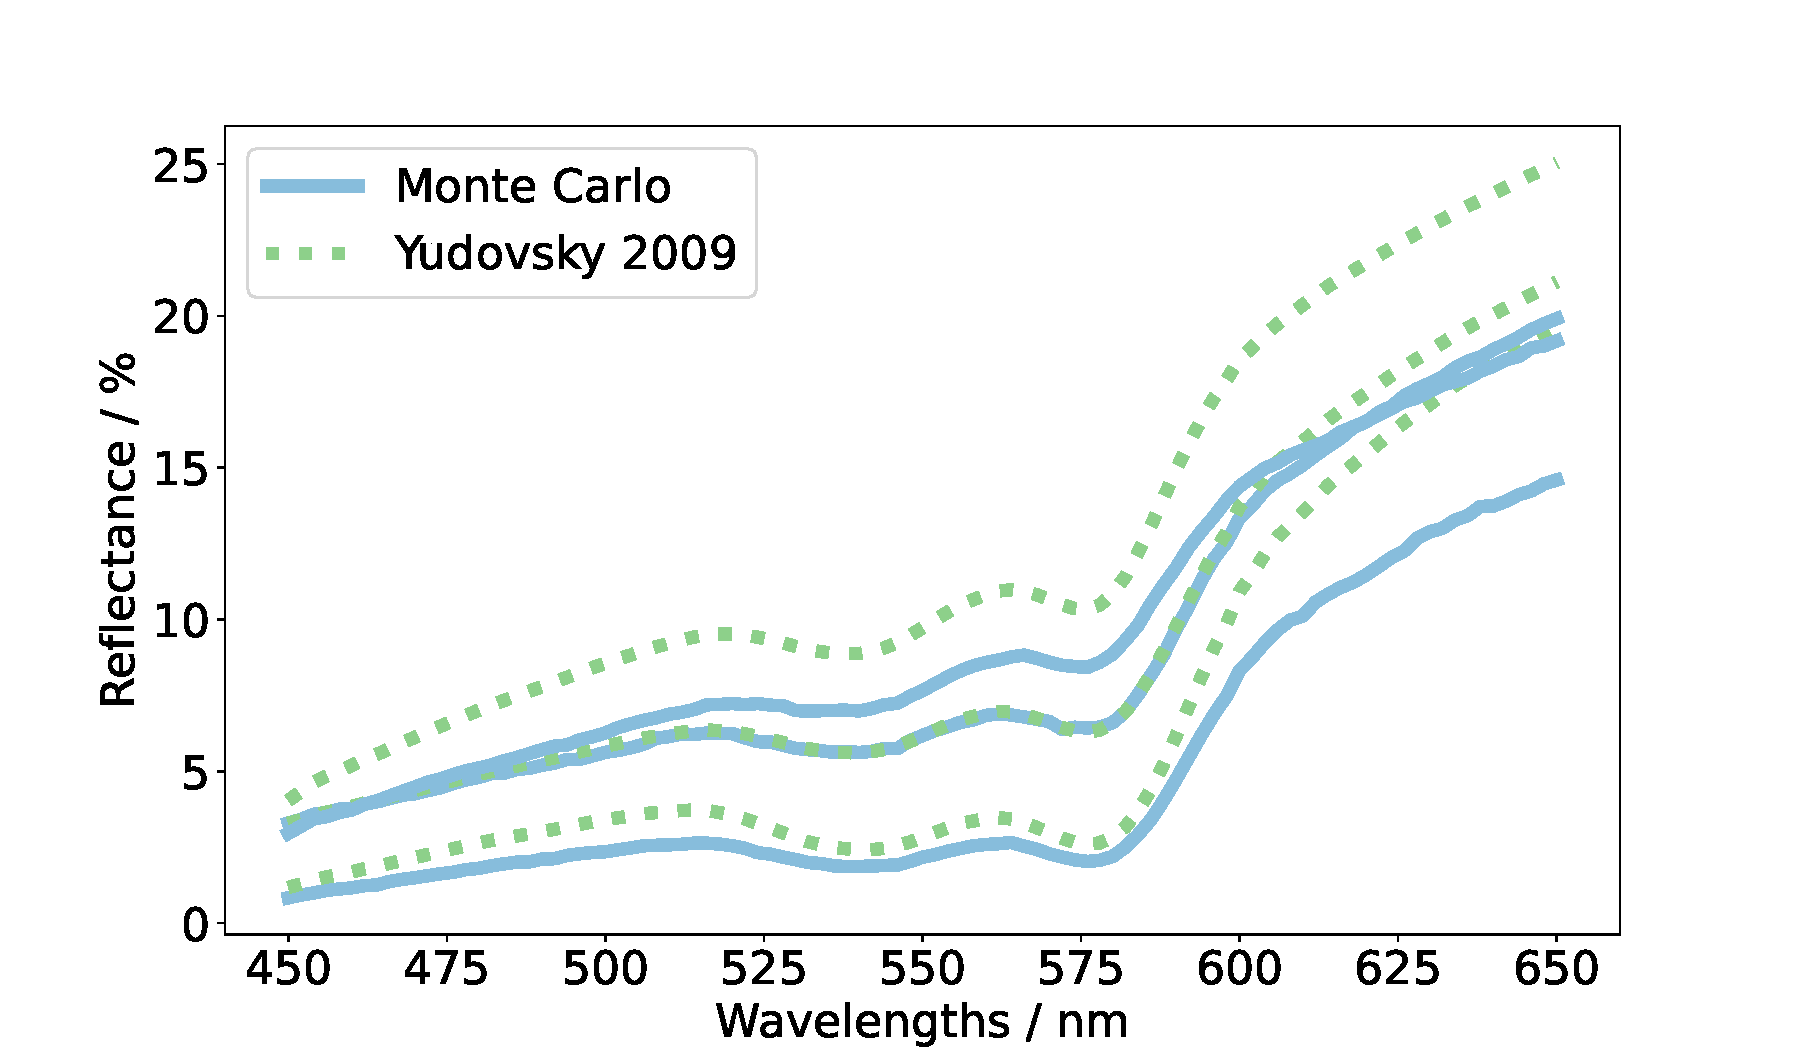
\includegraphics[width=\textwidth]{Compare_forwards_2_layer.pdf}
        \caption{Quantitative}
        \label{fig:egtwolayerMCforwards}
    \end{subfigure}
    \begin{subfigure}{0.49\textwidth}
        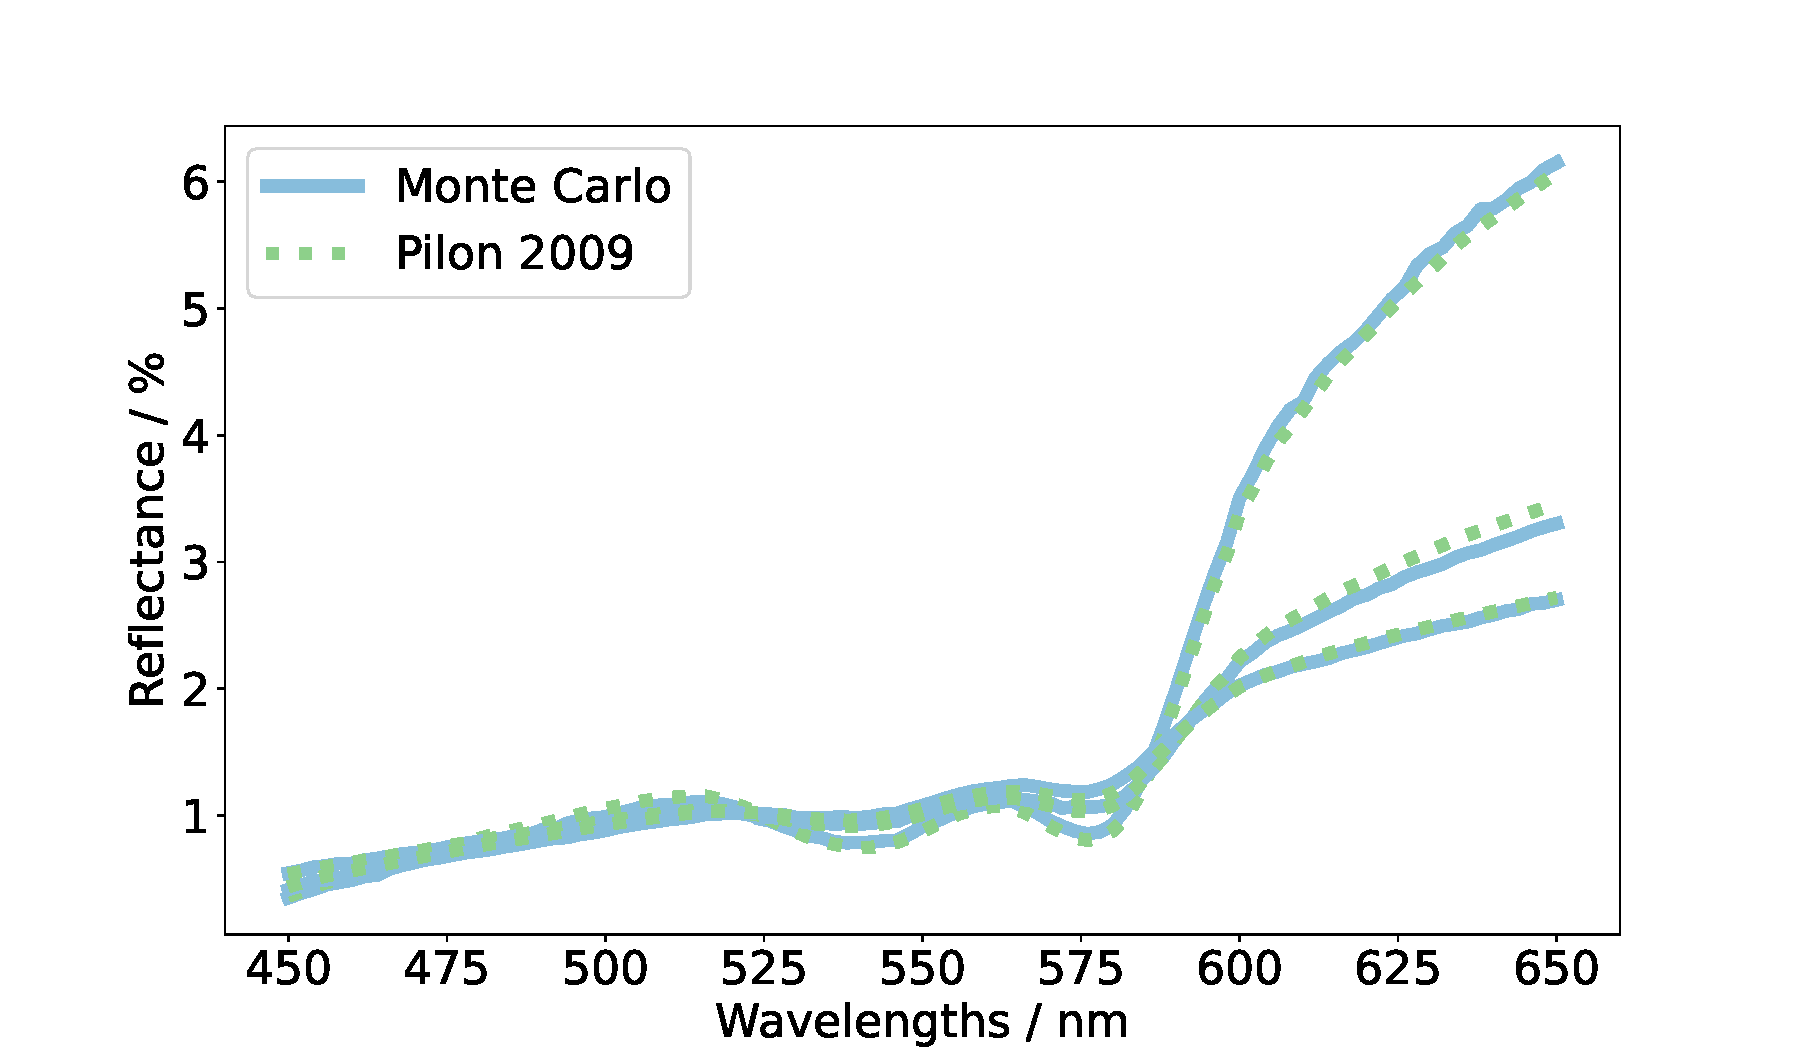
\includegraphics[width=\textwidth]{Compare_forwards_2_layer_norm.pdf}
        \caption{Relative}
        \label{fig:egtwolayerMCforwardsnorm}
    \end{subfigure}
    \begin{subfigure}{0.49\textwidth}
        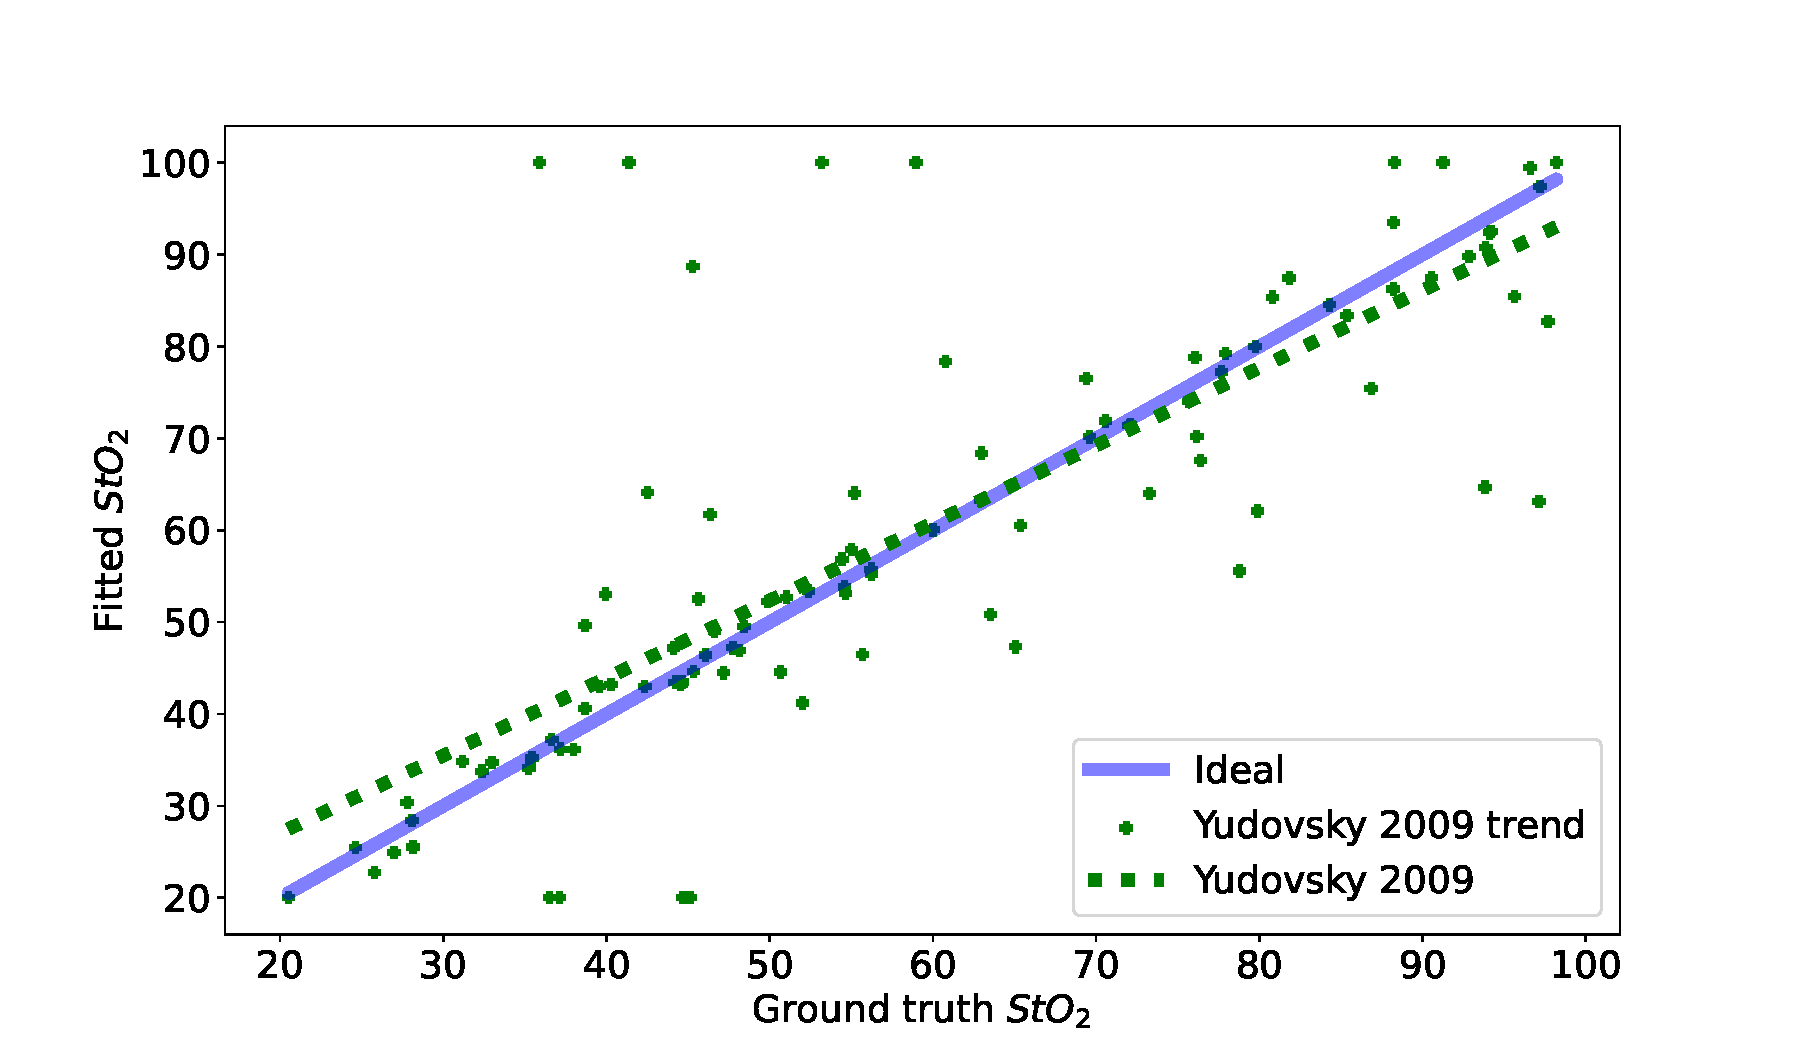
\includegraphics[width=\textwidth]{StO2_twolayer_MC.pdf}
        \caption{Quantitative}
        \label{fig:egparamsStO2MC}
    \end{subfigure}
    \begin{subfigure}{0.49\textwidth}
        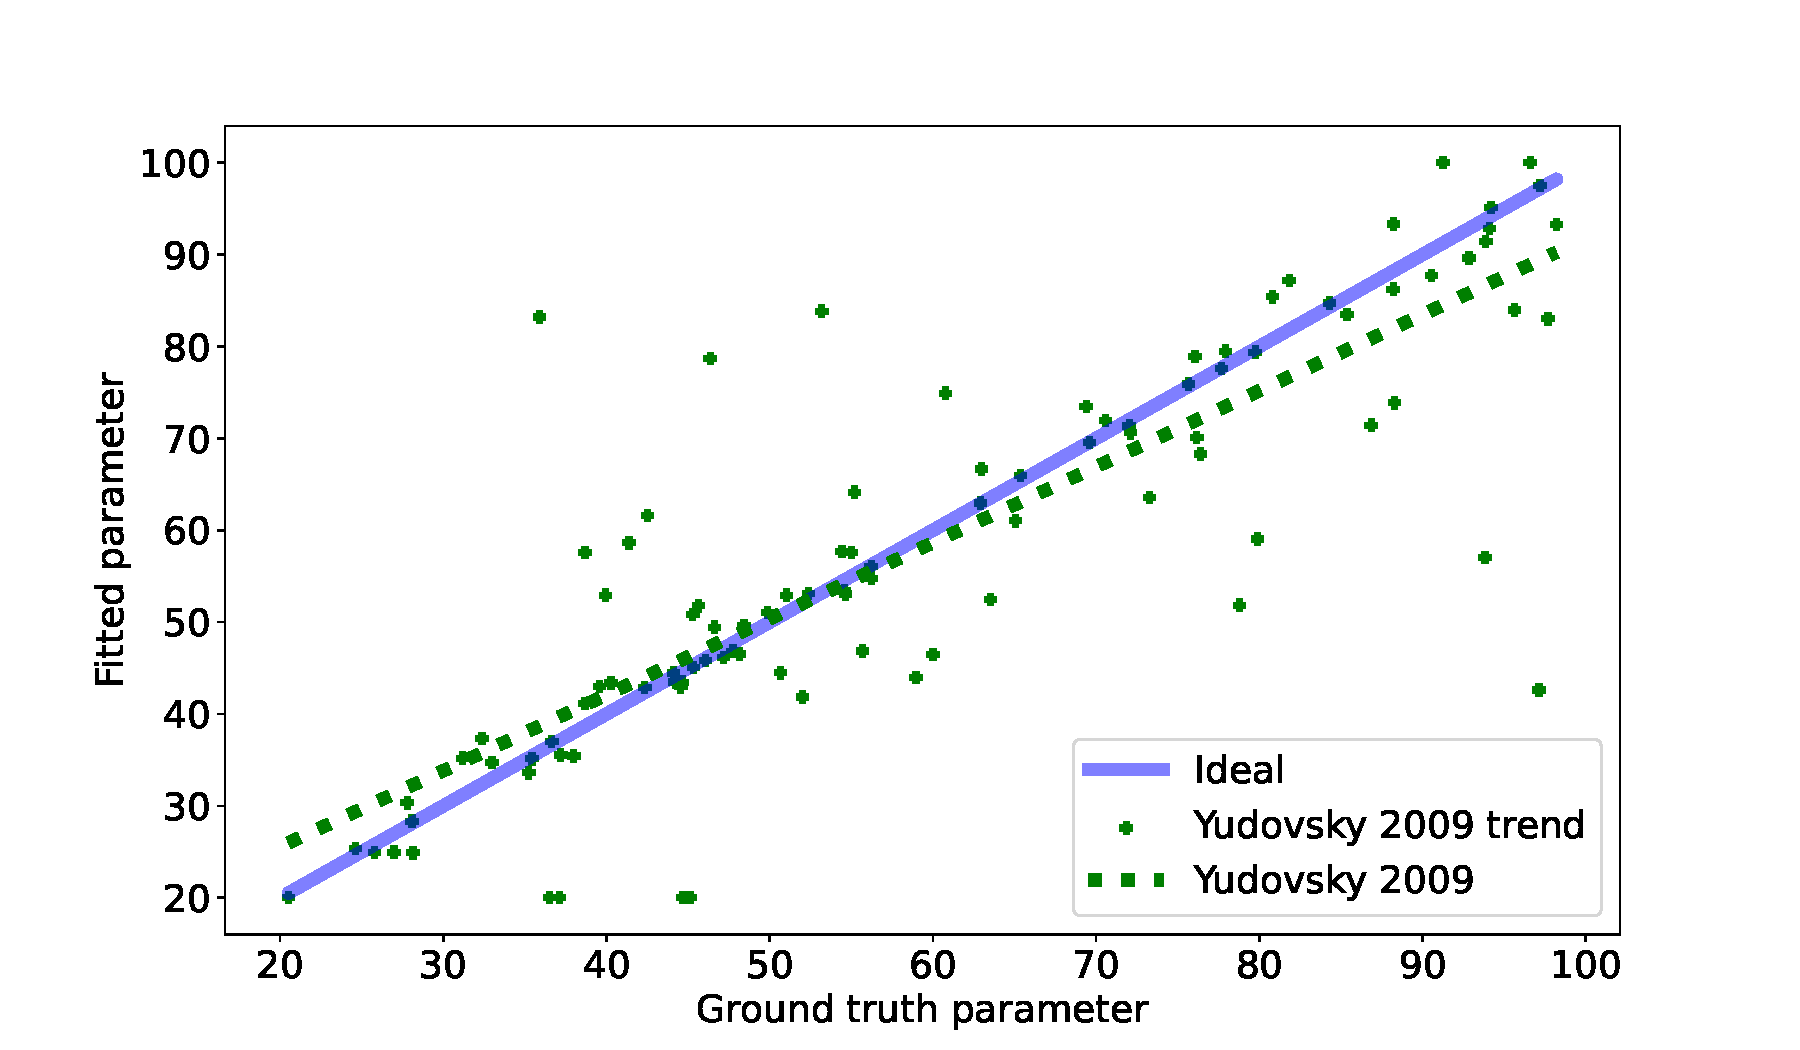
\includegraphics[width=\textwidth]{StO2_twolayer_MC_norm.pdf}
        \caption{Relative}
        \label{fig:egparamsStO2MCnorm}
    \end{subfigure}
    \begin{subfigure}{0.49\textwidth}
        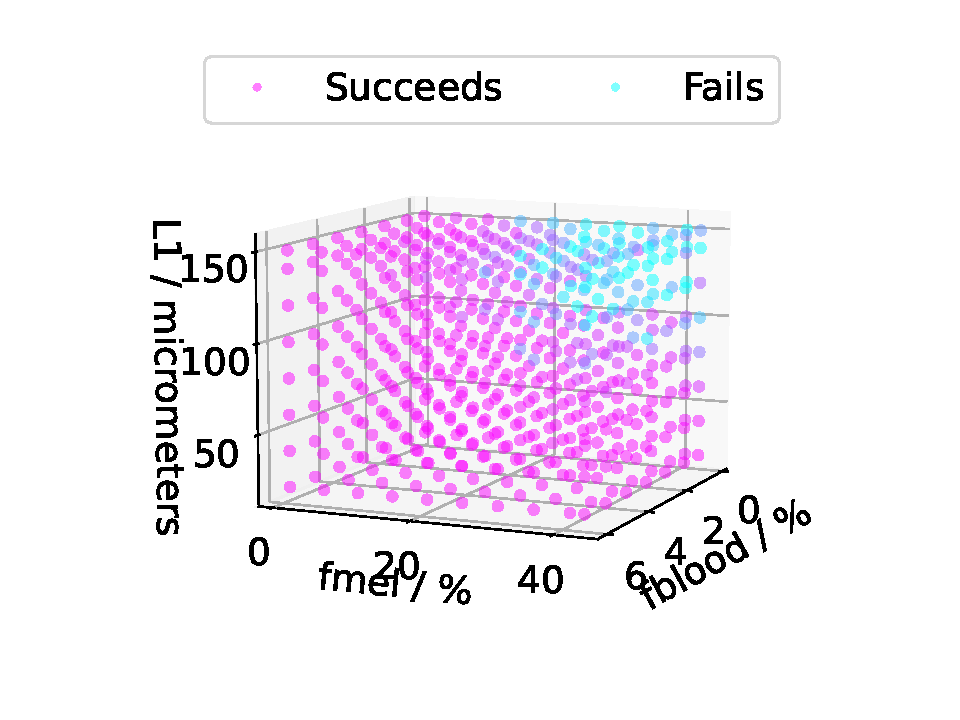
\includegraphics[width=\textwidth]{2layer_parameter_exploration.pdf}
        \caption{Quantitative}
        \label{fig:egparamsfailureMC}
    \end{subfigure}
    \begin{subfigure}{0.49\textwidth}
        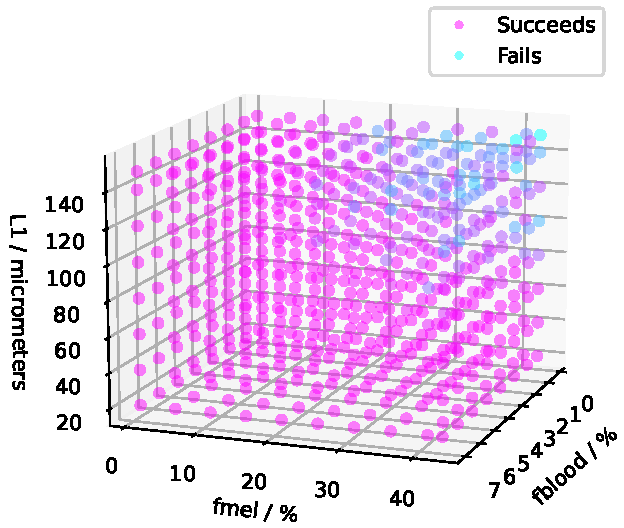
\includegraphics[width=\textwidth]{2layer_parameter_exploration_norm.pdf}
        \caption{Relative}
        \label{fig:egparamsfailureMCnorm}
    \end{subfigure}
    \caption{Top: Demonstration of the variability of quality of fit between the Yudovsky 2009 two-layer model and Monte Carlo simulated diffuse spectra when using the same ground truth parameters for quantitative (left) or relative (right) data. Middle: Example $StO_2$ recovery from fitting Yudovsky 2009 two-layer model to Monte Carlo simulated diffuse reflectance and the associated linear regression line between the extracted and ground truth parameters for quantitative (left) or relative (right) data. Bottom: a depiction of the impact of 3 key physiological parameters on success of $StO_2$ extraction by visualising the Pearson $r$ correlation coefficient for the extracted $StO_2$ compared to the ground-truth for simulations with this range of parameters extracted using Yudovsky 2009 two-layer model for quantitative (left) or relative (right) data.}
    \label{fig:MC2layer}
\end{figure}

When fitting the model to the Monte Carlo dataset, the $a$, $b$, $StO_2$, $f_{blood}$, $f_{mel}$, and $L_1$ parameters are extracted and compared to the ground truth Monte Carlo inputs using a linear regression. The regression gradient $m$ and offset $c$ between these retrieved values and the ground truth counterparts, alongside the Pearson $r$ values (bold if $p<0.05$ which is considered significant), and the mean ($\pm$ standard deviation) absolute percentage errors are shown in \tabref{tb:doubleparamtrends}. An example of the fitted parameters compared to the ground truth parameters is shown for $StO_2$ in  \figref{fig:egparamsStO2MC} for quantitative data and  \figref{fig:egparamsStO2MCnorm} for relative data. This shows parameter extraction to be significantly poorer than for the single-layer model and parameter extraction from quantitative data performing similarly that of relative data for $StO_2$ but better for all others. 
\begin{table}[t]
    \centering
    \caption{The regression gradient $m$, offset $c$, Pearson $r$ (bold if $p<0.05$), and the mean ($\pm$ standard deviation) absolute percentage errors (APE) for each variable when extracted by fitting Yudovsky 2009 two-layer model to the quantitative or relative Monte-Carlo diffuse reflectance dataset. All presented to 3s.f.}
    \begin{tabular}{|c|c|cccc|}
        \hline
        Parameter & Quantitative & $m$ & $c$ & $r$ & Mean ($\pm$ Standard  \\
        & or Relative & (ideal =1) & (ideal = 0) & (ideal = 1) & deviation) APE (\%)\\
        \hline
        \multirow{2}{*}{$StO_2$} & Quantitative & 0.844 & 10.2 & \textbf{0.788} & 15.3($\pm$ 27.5) \\
        & Relative & 0.827 & 8.99 & \textbf{0.836} & 13.1($\pm$ 19.7) \\
        \hline
        \multirow{2}{*}{$f_{blood}$} & Quantitative & 0.948 & 0.270 & \textbf{0.852} & 24.0($\pm$ 23.9) \\
        & Relative & 0.784 & 0.216 & \textbf{0.672} & 32.4($\pm$ 27.8) \\
        \hline
        \multirow{2}{*}{$f_{mel}$} & Quantitative & 0.842 & 1.38 & \textbf{0.843} & 27.0($\pm$ 25.7) \\
        & Relative & 0.502 & 5.14 & \textbf{0.506} & 38.1($\pm$ 24.6) \\
        \hline
        \multirow{2}{*}{$L_1$} & Quantitative & 0.825 & 31.4 & \textbf{0.794} & 38.6($\pm$ 41.9) \\
         & Relative & 0.798 & 37.7 & \textbf{0.775} & 41.6($\pm$ 39.9) \\
        \hline
        \multirow{2}{*}{$a$} & Quantitative & 0.752 & 11.2 & \textbf{0.617} & 20.0($\pm$ 15.5) \\
        & Relative & 0.445 & 24.0 & \textbf{0.333} & 28.0($\pm$ 24.6) \\
        \hline
        \multirow{2}{*}{$b$} & Quantitative & 0.826 & 0.286 & \textbf{0.739} & 16.4($\pm$ 18.5) \\
        & Relative & 0.710 & 0.530 & \textbf{0.509} & 29.6($\pm$ 31.4) \\
        \hline
    \end{tabular}
    \label{tb:doubleparamtrends}
\end{table}
Graphs shown in \figref{fig:egparamsfailureMC} (quantitative) and \figref{fig:egparamsfailureMCnorm} (relative) demonstrate the impact of each parameter on model success for $StO_2$ parameter extraction when a singular ground truth scattering is fixed. This shows that the effect of $StO_2$ on the diffuse reflectance spectrum is masked by the melanin effect in areas of low $f_{blood}$, or high $L_1$ or $f_{mel}$ leading to poor $StO_2$ extraction in these areas. 
\FloatBarrier

\subsection{NIST}\label{sec:resultsNIST}
The Yudovsky two-layer model is fitted to a NIST skin total reflectance dataset. %The weighting function in \figref{fig:weighting} is used to ensure good fitting and a refractive index of 1.44 is assumed for tissue in the visible range \citep{Yudovsky2009}. 
There are no ground truth parameters for these measured spectra, however the $a$, $b$, $StO_2$, $f_{blood}$, $f_{mel}$, and $L_1$ parameters are extracted and the mean ($\pm$ standard deviation) is compared to expected values for healthy individuals~\citep{Jacques2013, VanManen2021, Nishidate2011, Lintzeri2022} in \tabref{tb:NISTparams} for quantitative (Q) and relative (R) data. This demonstrates that overall fitting to relative data performs better than quantitative data, however neither is able to recover $StO_2$ well. 
\begin{figure}[h]
    \centering
    \begin{subfigure}{0.49\textwidth}
        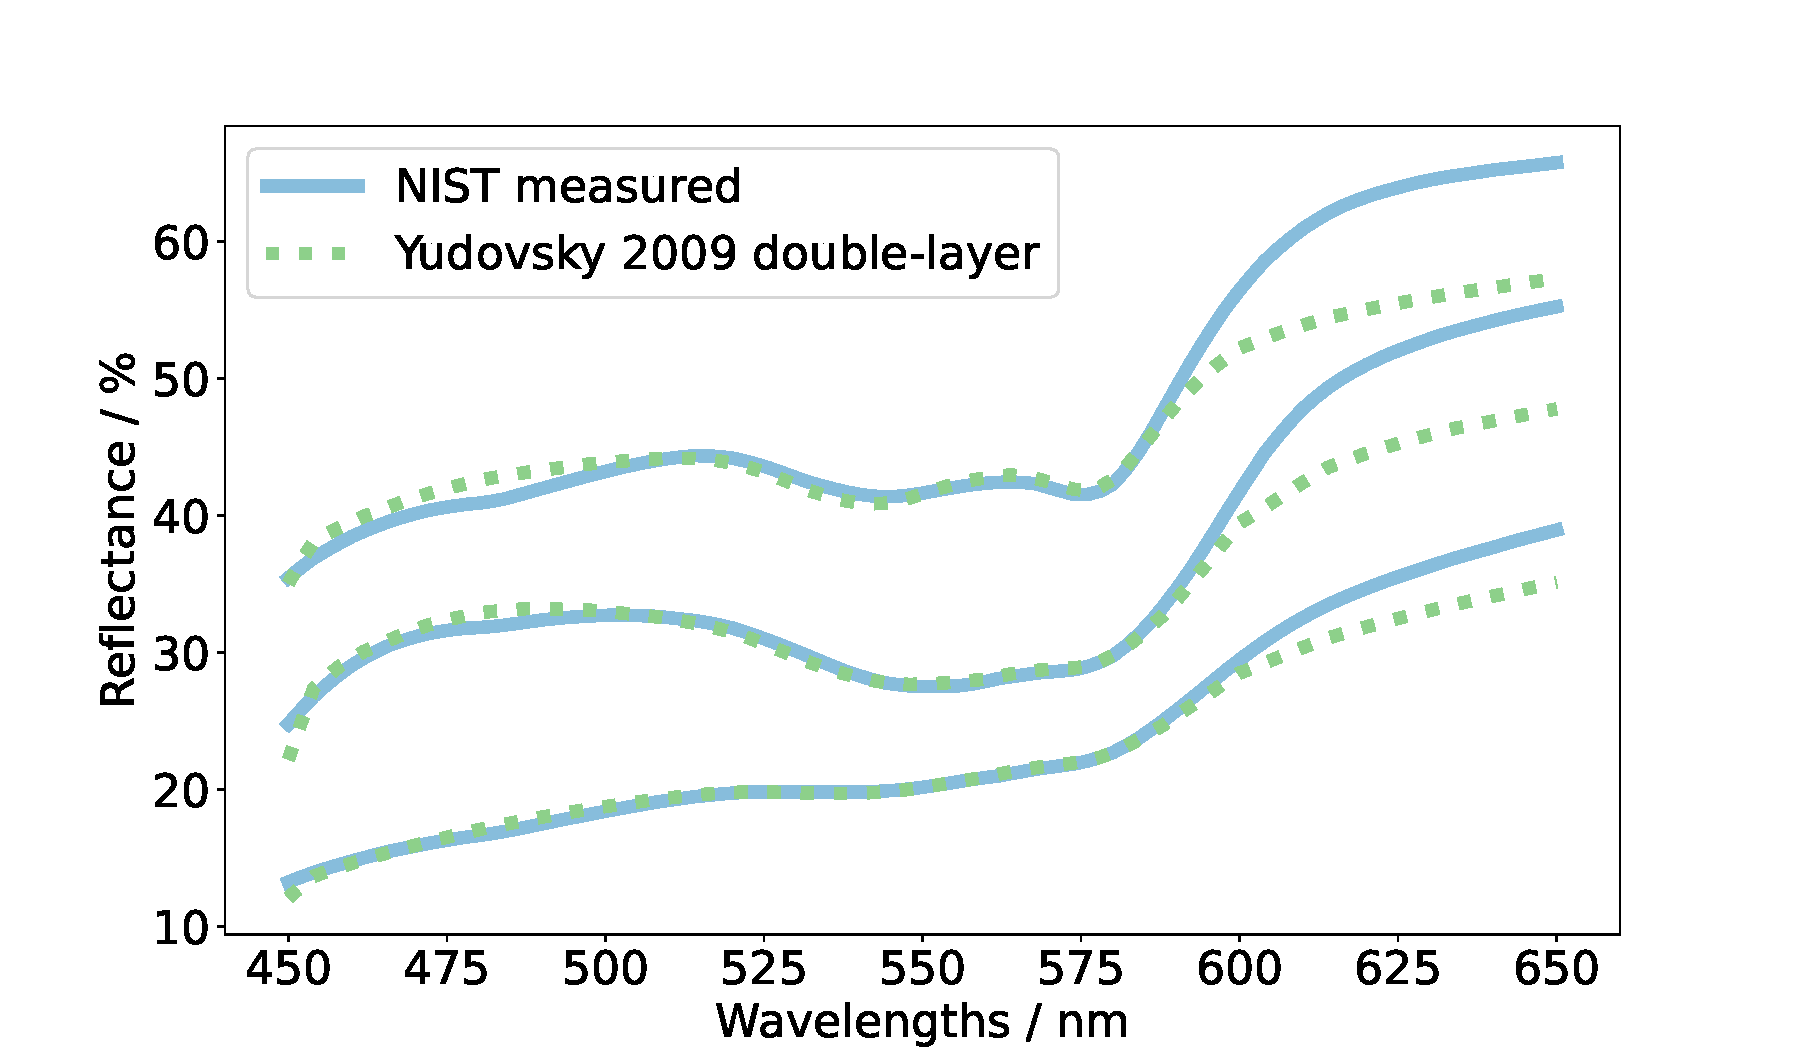
\includegraphics[width=\textwidth]{NIST_Eg.pdf}
        \caption{Quantitative}
        \label{fig:egspectraNIST}
    \end{subfigure}
    \begin{subfigure}{0.49\textwidth}
        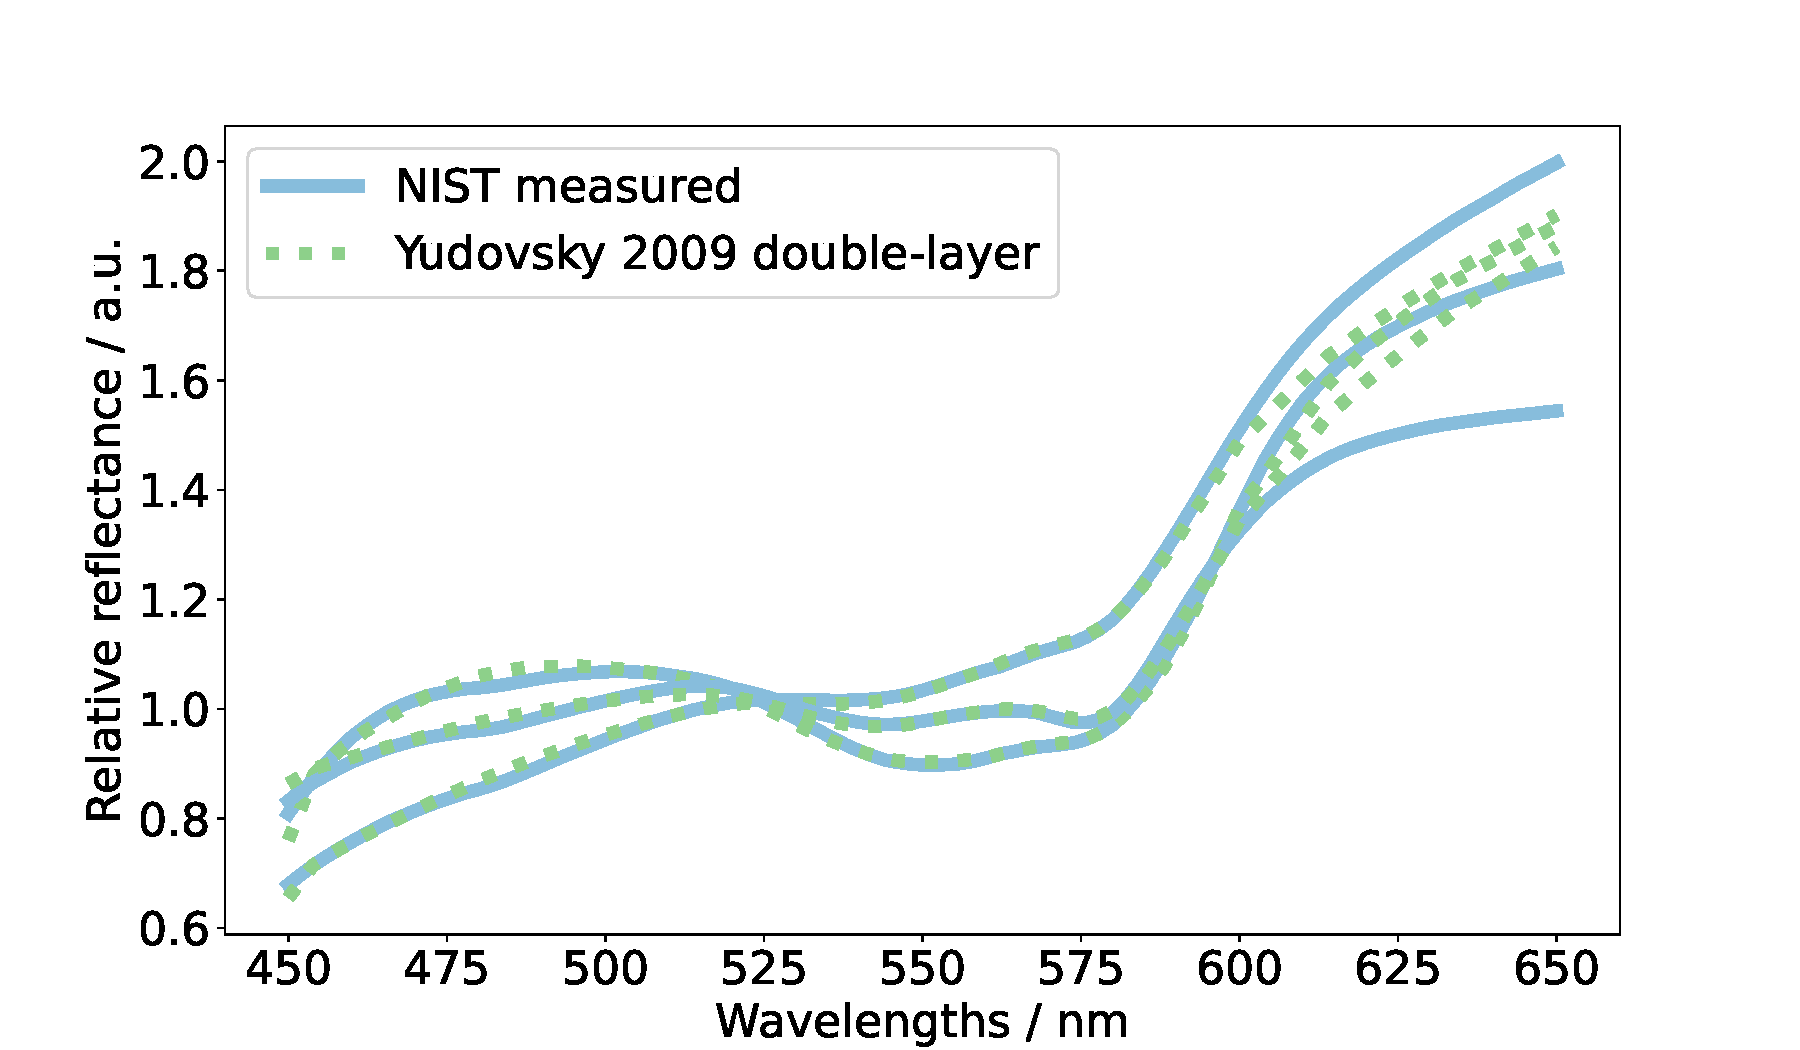
\includegraphics[width=\textwidth]{NIST_Eg_norm.pdf}
        \caption{Relative}
        \label{fig:egspectraNISTnorm}
    \end{subfigure}
    \begin{subfigure}{0.49\textwidth}
        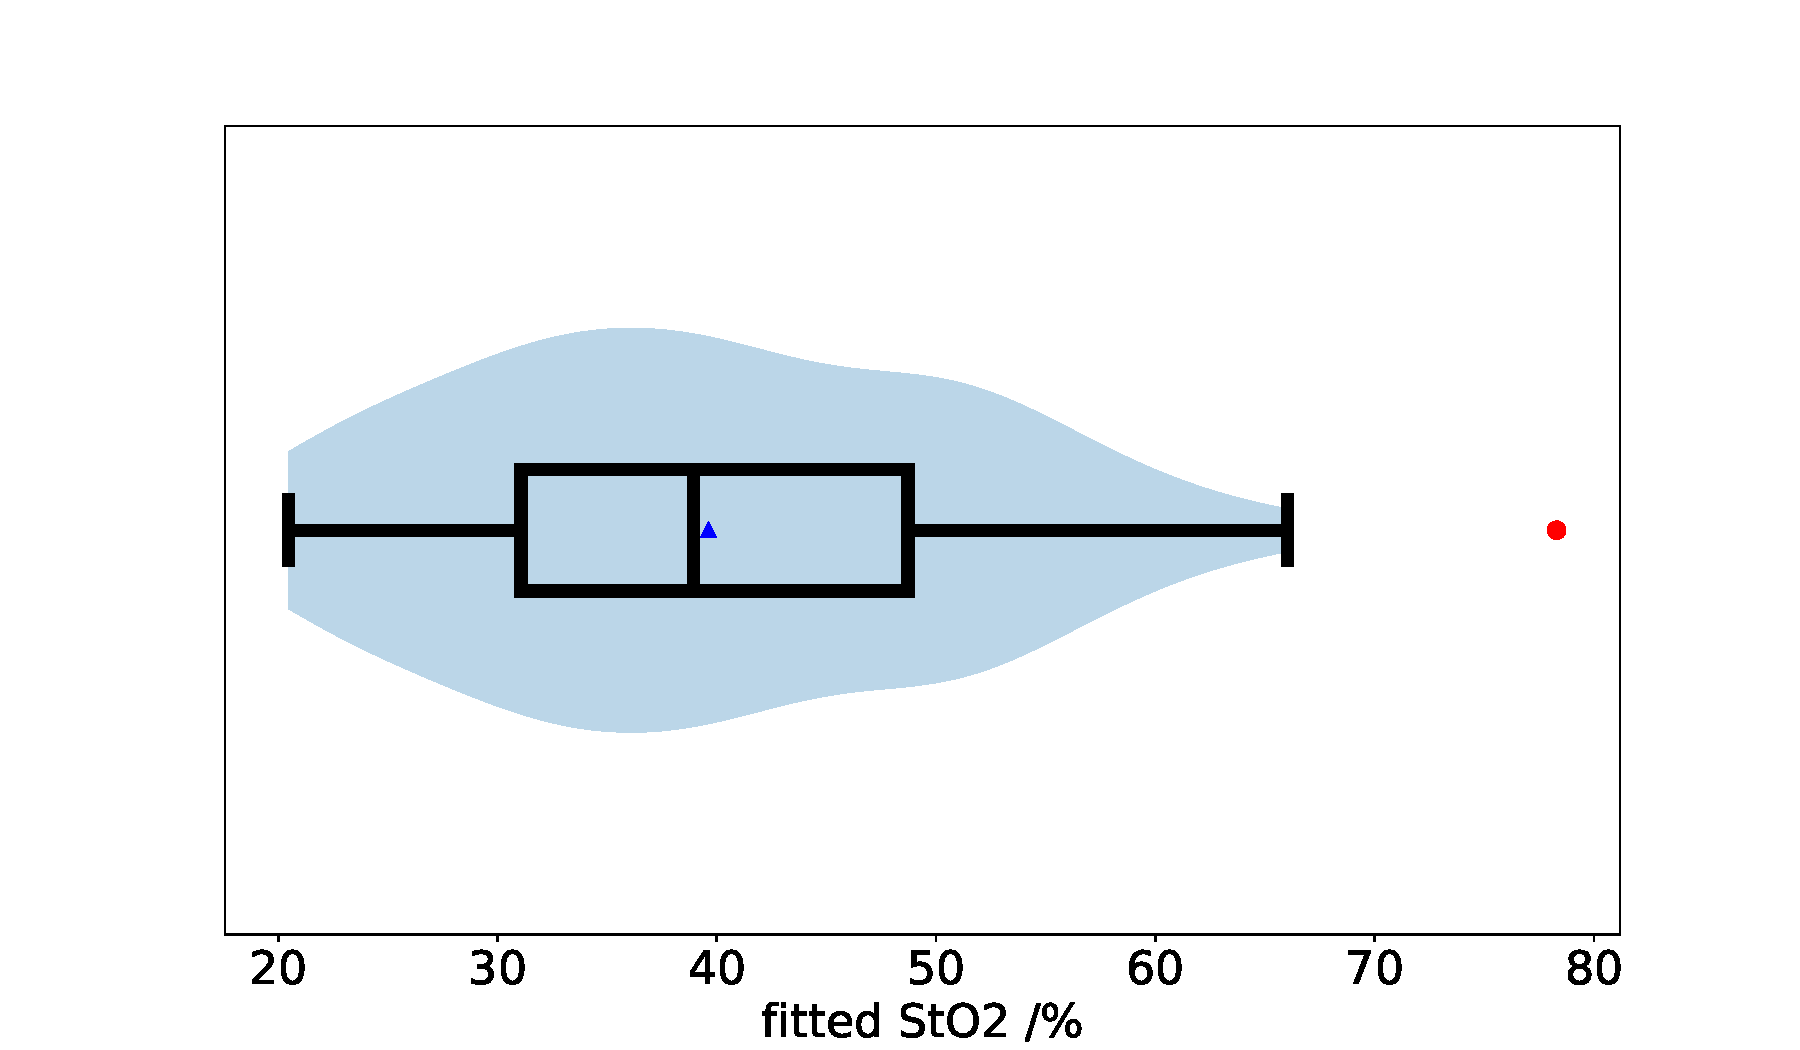
\includegraphics[width=\textwidth]{StO2_boxplot.pdf}
        \caption{Quantitative}
        \label{fig:egparamStO2NIST}
    \end{subfigure}
    \begin{subfigure}{0.49\textwidth}
        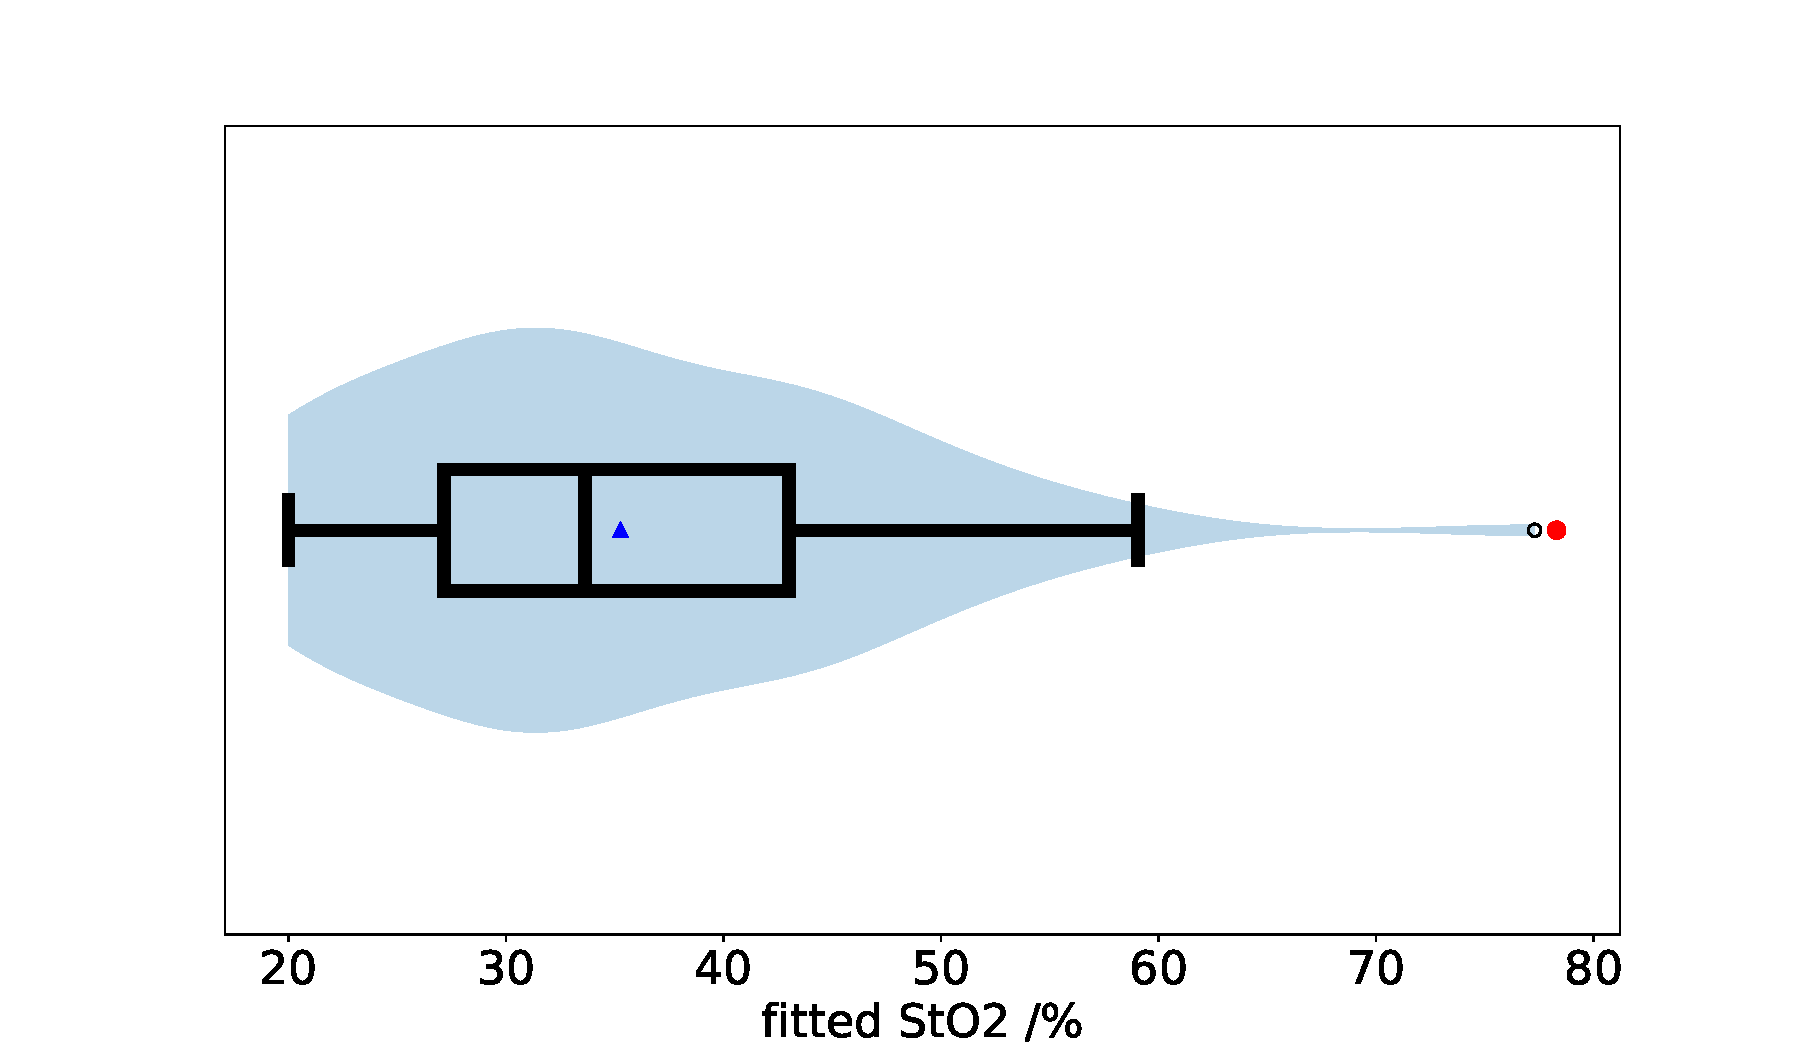
\includegraphics[width=\textwidth]{StO2_boxplot_norm.pdf}
        \caption{Relative}
        \label{fig:egparamStO2NISTnorm}
    \end{subfigure}
    \caption{Top: Examples of the Yudovsky 2009 two-layer model fitted to NIST skin total reflectance spectra (\figref{fig:egspectraNIST}) for quantitative (left) or relative (right) data. Bottom: Box and violin plots displaying the retrieved $StO_2$ parameters from fitting the Yudovsky 2009 two-layer model to the mean NIST skin spectra, where the triangle shows the mean of the fitted $StO_2$ and the circle shows a literature healthy dermis $StO_2$ value~\citep{VanManen2021} for quantitative (left) or relative (right) data.}
    \label{fig:NIST}
\end{figure}
\begin{table}[h]
    \centering
    \caption{The mean and standard deviation for each variable when extracted by fitting Yudovsky 2009 two-layer model to the quantitative or relative (Q or R) NIST skin reflectance dataset, compared to literature parameters for healthy individuals. All presented to 3s.f.}
    \begin{tabular}{|c|ccc|ccc|}
        \hline
         & \multicolumn{3}{c}{Extracted from NIST dataset} & \multicolumn{3}{|c|}{Literature} \\
        \cline{2-7}
         \rot{Parameter} & \multirow{2}{*}{Q or R} & \multirow{2}{*}{Mean} & Standard & \multirow{2}{*}{Mean} & Standard & \multirow{2}{*}{Source} \\
         &  &  & deviation &  & deviation &  \\
        \hline
        $StO_2$ & Q & 39.6 & 11.1 & \multirow{2}{*}{78.3, 71} & \multirow{2}{*}{12.9, 16} & \cite{VanManen2021}, \\ %van manen http://dx.doi.org/10.21037/qims-21-46
        (\%) & R & 35.3 & 10.9 & & & \cite{Nishidate2011} \\ %Noninvasive imaging of human skin hemodynamicsusing a digital red-green-blue camera
        \hline
        $f_{blood}$ & Q & 0.643 & 0.588 & \multirow{2}{*}{1.1} & \multirow{2}{*}{0.4} & \multirow{2}{*}{\cite{Nishidate2011}} \\ %Noninvasive imaging of human skin hemodynamicsusing a digital red-green-blue camera
        (\%) & R & 2.72 & 1.82 & & & \\
        \hline
        $f_{mel}$ & Q & 5.39 & 6.09 & \multirow{2}{*}{4.3} & \multirow{2}{*}{1.2} & \multirow{2}{*}{\cite{Nishidate2011}} \\ %Noninvasive imaging of human skin hemodynamicsusing a digital red-green-blue camera
        (\%) & R & 3.61 & 2.95 & & &  \\
        \hline
        $L_1$ & Q & 44.3 & 24.3 & \multirow{2}{*}{75.5} & \multirow{2}{*}{N/A} & \multirow{2}{*}{\cite{Lintzeri2022}} \\ %https://www.webofscience.com/wos/woscc/full-record/WOS:000782026000001
        ($\mu$m) & R & 146 & 15.2 & & &  \\
        \hline
        $a$ & Q & 70.0 & 2.91$\times 10^{-8}$ & \multirow{2}{*}{46.0} & \multirow{2}{*}{13.7} & \multirow{2}{*}{\cite{Jacques2013}} \\ %Jacques review
        (\textrm{$cm^{-1}$}) & R & 47.9 & 13.0 & & &  \\
        \hline
        $b$ & Q & 1.57 & 0.622 & \multirow{2}{*}{1.421} & \multirow{2}{*}{0.517} & \multirow{2}{*}{\cite{Jacques2013}} \\ %Jacques review
        (a.u.) & R & 2.45 & 0.208 & & &  \\
        \hline
    \end{tabular}
    \label{tb:NISTparams}
\end{table}
Examples of the fitted model to some NIST spectra and box plots overlaid with a violin plots for $StO_2$ are shown in \figref{fig:NIST} for quantitative and relative data. 
\FloatBarrier

\section{Discussion and future work}\label{sec:discussion2}
Whilst the Yudovsky single-layer model has shown excellent spectral prediction in our previous work~\citep{Bahl2023a}, this quality cannot be replicated by the Yudovsky two-layer model when compared with two-layer Monte Carlo simulations. It is clear that there is significant variability in the performance of the two-layer Yudovsky model. This is noted both in the variability of fits to the Monte Carlo spectra and quality of the parameter extraction. The Yudovskly two-layer model spectral prediction is vastly improved when modelling relative data compared to quantitative data as shown by the reduction in $NRMSE$ and the visual fits, however this improvement is not clearly seen in parameter extraction from the Monte Carlo data. The most robust parameter extraction from this model is for $StO_2$. Leveraging this, the weaknesses of this model can be shown to be in regions of high $L_1$, high $f_{mel}$, and low $f_{blood}$. This follows intuition that in regions where the melanin impact in the epidermis is significant, it "masks" a low haemoglobin impact from the dermis. For this reason, this model should be used with caution as it has limited use in the region of failure identified.

Whilst this model appears to fit well to NIST skin experimental data when using a least-squares fitting routine, the parameters it returns are largely different to previous literature values for healthy individuals. The dermal layer is modelled identically to the single layer model which has been shown to perform well with well-characterised experimental data~\citep{Bahl2023a}, suggesting that there are interactions between layers, biological components that are not appropriately accounted for, or that the optical properties of these tissue types are not well characterised.  

This work should be viewed in light of it's limitations which include the lack of ground-truth parameters for the NIST skin dataset. It is challenging to obtain reliable ground-truth values for any in-vivo skin measurements so the results from this model's parameter extraction cannot be quantitatively evaluated easily. The $StO_2$ extraction methodologies used to obtain the quoted literature values are also associated with some limitations. \citet{Nishidate2011} trained a deep learning model using Monte Carlo simulations, however these simulations use a fixed layer thickness for epidermis and dermis and a single wavelength-dependent reduced scattering coefficient which may cause inaccuracies in the recovered physiological parameters from the in vivo data since these values are not fixed in biological samples. This deep learning model is also trained on noiseless simulations and, whilst the in vivo data was processed to reduce noise, some may remain. \citet{VanManen2021}, however, uses a modified Beer-Lambert-based model which simplifies the modelling of the anatomically layered structure of skin to a single layer. In both cases, these methods have not been validated with phantoms with known ground-truth so the precision and accuracy of the extracted parameters are unknown. For this reason, these comparisons may be flawed and further research using phantoms with known ground-truth values should be conducted.

In conclusion, this work demonstrates that the two-layer Yudovsky model does not perform with the same quality as the single-layer model. Combining this with the parameters extracted from the NIST dataset which do not correspond to other literature values and the failure regions depicted, demonstrates that this model should be used with caution. 

Future work should include investigation of the epidermis, similarly to investigation of the single-layer models with the dermis, and interaction between the layers to improve this model. This model could also be tested with layered tissue-mimicking optical phantoms with known ground truth parameters to allow full quantitative evaluation of the model performance with experimental data. 
%After improvement of the performance with experimental data, this model could be adapted for use with hyperspectral imaging cameras which may not have as densely sampled spectra, as these have been shown to be likely methods of obtaining these diffuse reflectance spectra intra-operatively \citep{Clancy2020}. 

In the context of this thesis, this model would be relevant for use within the brain. Here some of the layered structures may not have absorbing chromophores as powerful as melanin, e.g. Pia Mater, so it is more likely the parameters of these tissues will lie within the successful region of parameter space where both layers can be characterised well. For this reason this model is investigated further in Chapter~\ref{chap:HSImodel}, however future work should include the exclusion of highly absorbing upper layers for this work. 

% \bibliography{Paper3}
% \bibliographystyle{spiejour}

% \include{supplementary.tex}

% \end{document}
\clearpage
\begin{subappendices}
    \section{Appendices investigating two layer model using uniform wavelength weighting}\label{ap:2layeruniform}
This section presents a similar inverse problem fitting analysis to the results presented in Chapter~\ref{chap:2layer}, however the wavelength weighting used here is uniform. There are limited changes to the conclusions so further discussion is not provided, however it should be noted that the visual fitting of the 525-585nm of the NIST spectra is worsened using this configuration.

\subsection{Simulated data}
\begin{figure}[htbp]
    \centering
    \begin{subfigure}{0.49\textwidth}
        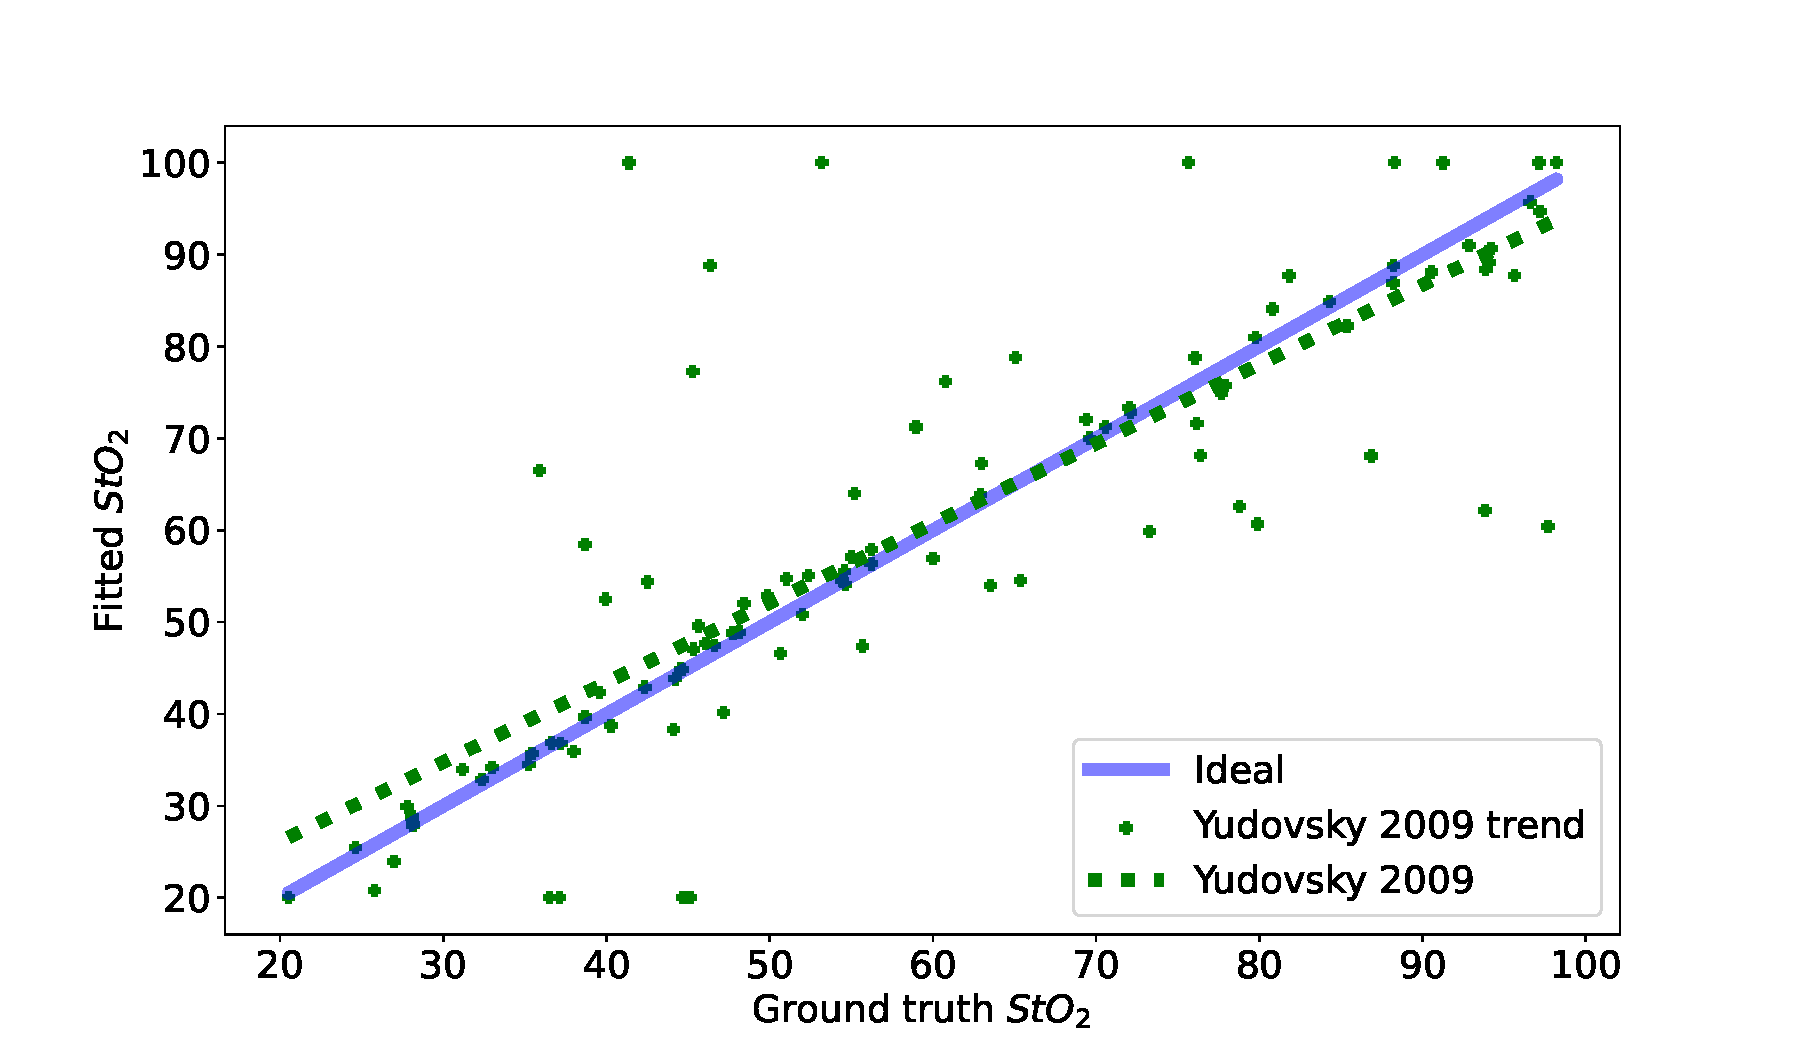
\includegraphics[width=\textwidth]{StO2_twolayer_MC_uniform.pdf}
        \caption{Quantitative}
        \label{fig:egparamsStO2MCu}
    \end{subfigure}
    \begin{subfigure}{0.49\textwidth}
        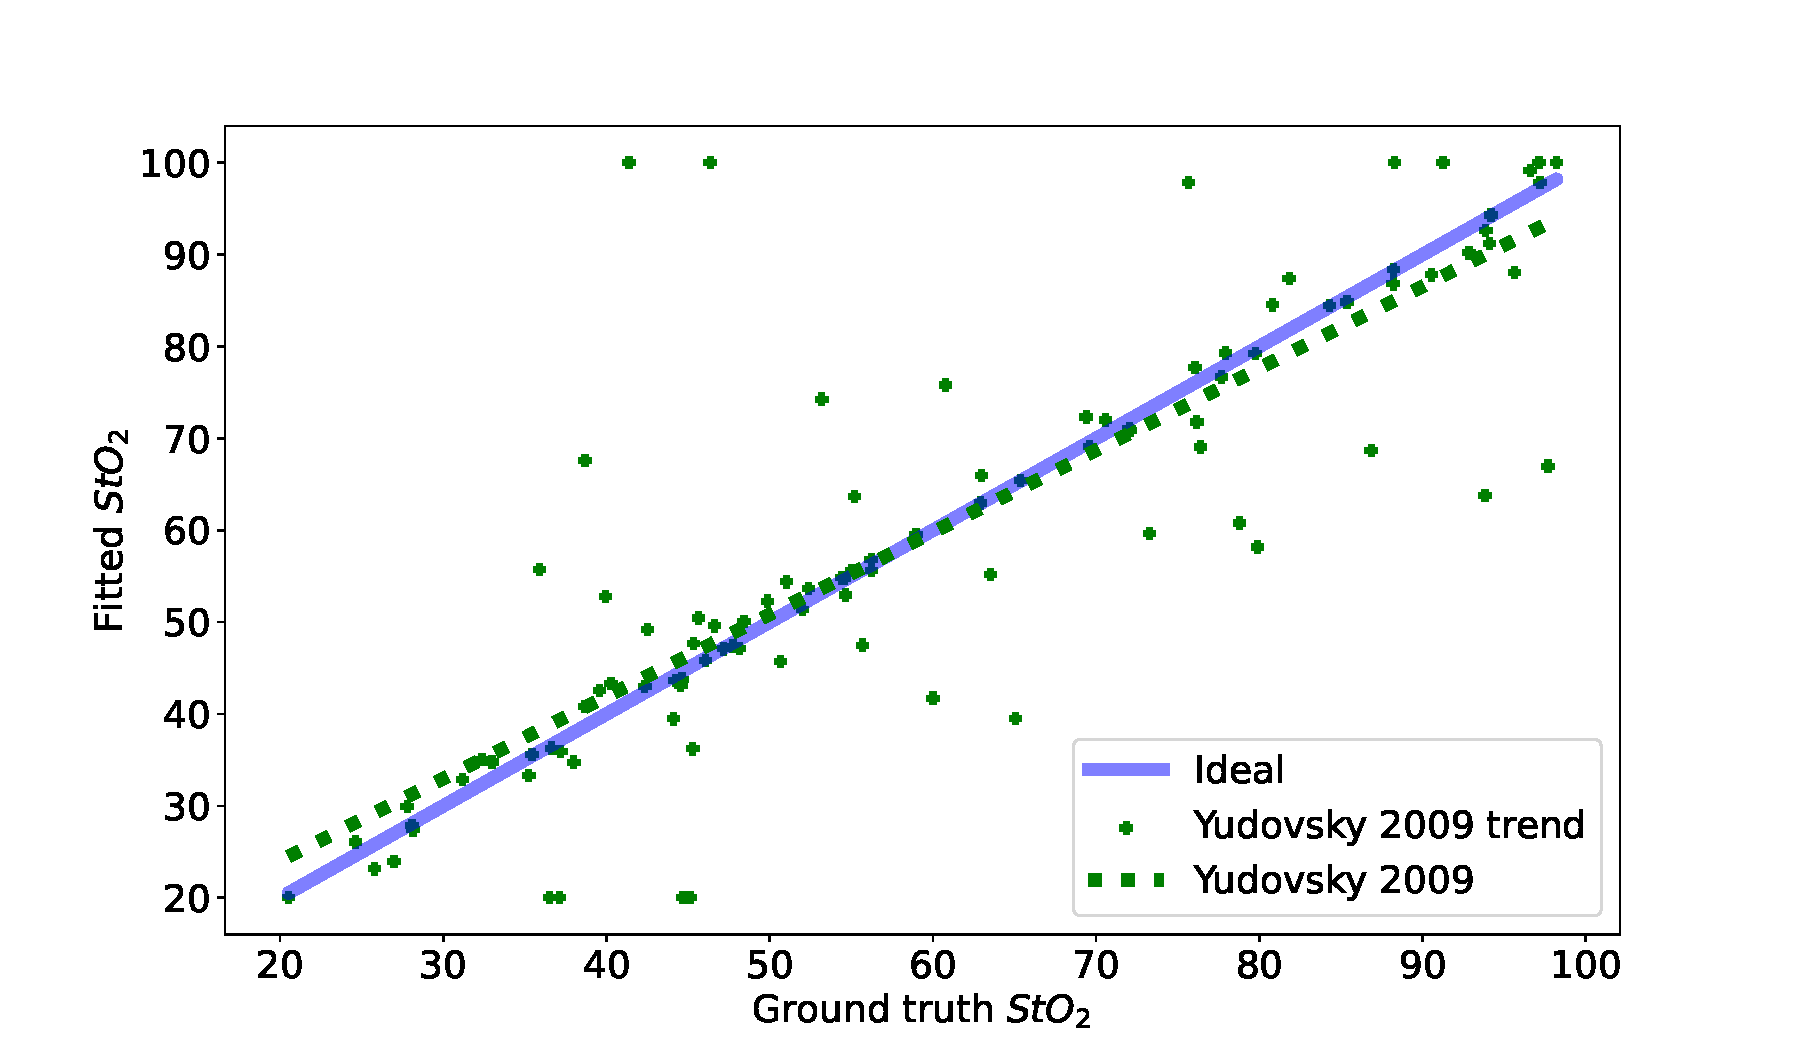
\includegraphics[width=\textwidth]{StO2_twolayer_MC_norm_uniform.pdf}
        \caption{Relative}
        \label{fig:egparamsStO2MCnormu}
    \end{subfigure}
    \begin{subfigure}{0.49\textwidth}
        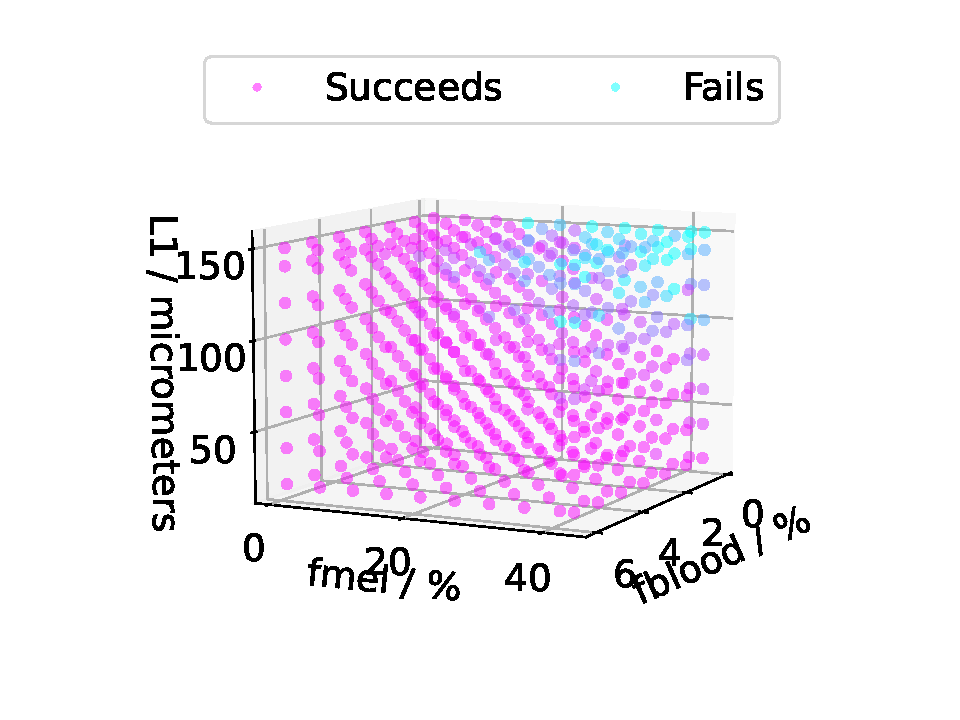
\includegraphics[width=\textwidth]{2layer_parameter_exploration_uniform.pdf}
        \caption{Quantitative}
        \label{fig:egparamsfailureMCu}
    \end{subfigure}
    \begin{subfigure}{0.49\textwidth}
        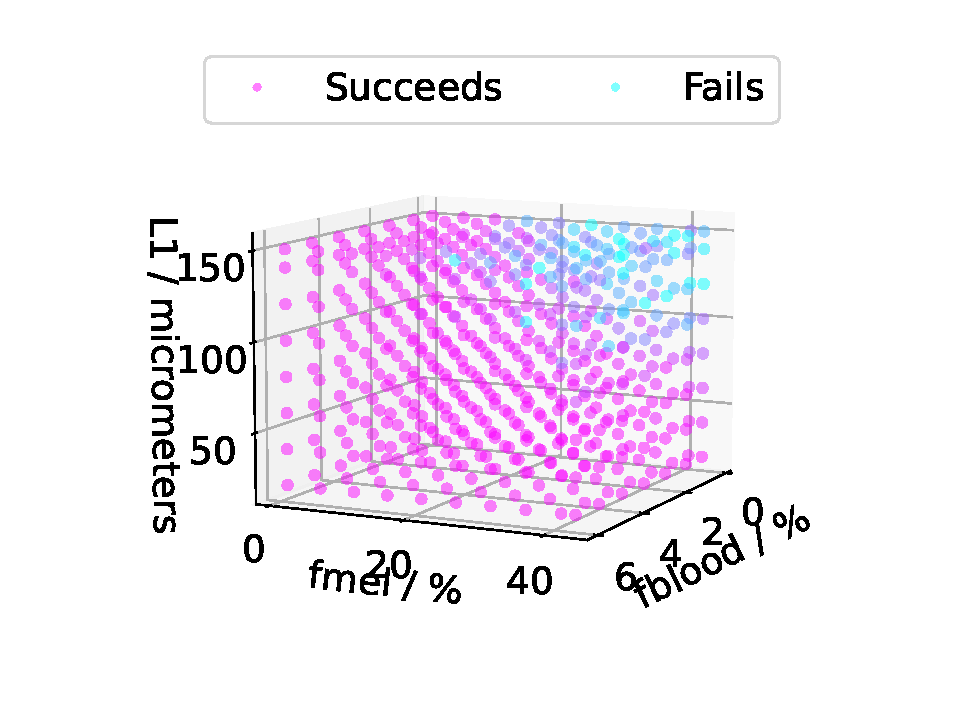
\includegraphics[width=\textwidth]{2layer_parameter_norm_uniform.pdf}
        \caption{Relative}
        \label{fig:egparamsfailureMCnormu}
    \end{subfigure}
    \caption{Top: Example $StO_2$ recovery from fitting Yudovsky 2009 two layer model to Monte Carlo simulated diffuse reflectance and the associated linear regression line between the extracted and ground truth parameters for quantitative (left) or relative (right) data. Bottom: a depiction of the impact of 3 key physiological parameters on success of $StO_2$ extraction by visualising the Pearson $r$ correlation coefficient for the extracted $StO_2$ compared to the ground-truth for simulations with this range of parameters extracted using Yudovsky 2009 two-layer model for quantitative (left) or relative (right) data.}
    \label{fig:MC2layeruniform}
\end{figure}

\begin{table}[h]
    \centering
    \caption{The regression gradient $m$, offset $c$, Pearson $r$ (bold if $p<0.05$), and the mean ($\pm$ standard deviation) absolute percentage errors (APE) for each variable when extracted by fitting Yudovsky 2009 two layer model to the quantitative (Q) or relative (R) Monte-Carlo diffuse reflectance dataset with uniform weighting of wavelengths. All presented to 3s.f.}
    \begin{tabular}{|c|c|cccc|}
        \hline
        Parameter & Q or R & $m$ & $c$ & $r$ & mean ($\pm$ standard  \\
        &  & (ideal =1) & (ideal = 0) & (ideal = 1) & deviation) APE (\%)\\
        \hline
        \multirow{2}{*}{$StO_2$} & Q & 0.866 & 8.81 & \textbf{0.821} & 14.2($\pm$ 23.1) \\
        & R & 0.893 & 6.18 & \textbf{0.842} & 13.0($\pm$ 22.2) \\
        \hline
        \multirow{2}{*}{$f_{blood}$} & Q & 0.956 & 0.160 & \textbf{0.856} & 25.1($\pm$ 25.3) \\
        & R & 0.839 & 3.35$\times 10^{-2}$ & \textbf{0.706} & 30.9($\pm$ 25.9) \\
        \hline
        \multirow{2}{*}{$f_{mel}$} & Q & 0.838 & 1.17 & \textbf{0.875} & 23.9($\pm$ 18.6) \\
        & R & 0.497 & 5.45 & \textbf{0.531} & 35.4($\pm$ 25.0) \\
        \hline
        \multirow{2}{*}{$L_1$} & Q & 0.840 & 31.3 & \textbf{0.824} & 37.1($\pm$ 39.1) \\
         & R & 0.827 & 34.9 & \textbf{0.805} & 39.0($\pm$ 36.6) \\
        \hline
        \multirow{2}{*}{$a$} & Q & 0.682 & 13.3 & \textbf{0.586} & 19.4($\pm$ 14.6) \\
        & R & 0.515 & 20.5 & \textbf{0.389} & 26.1($\pm$ 22.3) \\
        \hline
        \multirow{2}{*}{$b$} & Q & 0.804 & 0.338 & \textbf{0.781} & 14.2($\pm$ 16.4) \\
        & R & 0.729 & 0.521 & \textbf{0.586} & 25.1($\pm$ 26.7) \\
        \hline
    \end{tabular}
    \label{tb:doubleparamtrendsuniform}
\end{table}
\FloatBarrier

\subsection{NIST}
\begin{figure}[h]
    \centering
    \begin{subfigure}{0.49\textwidth}
        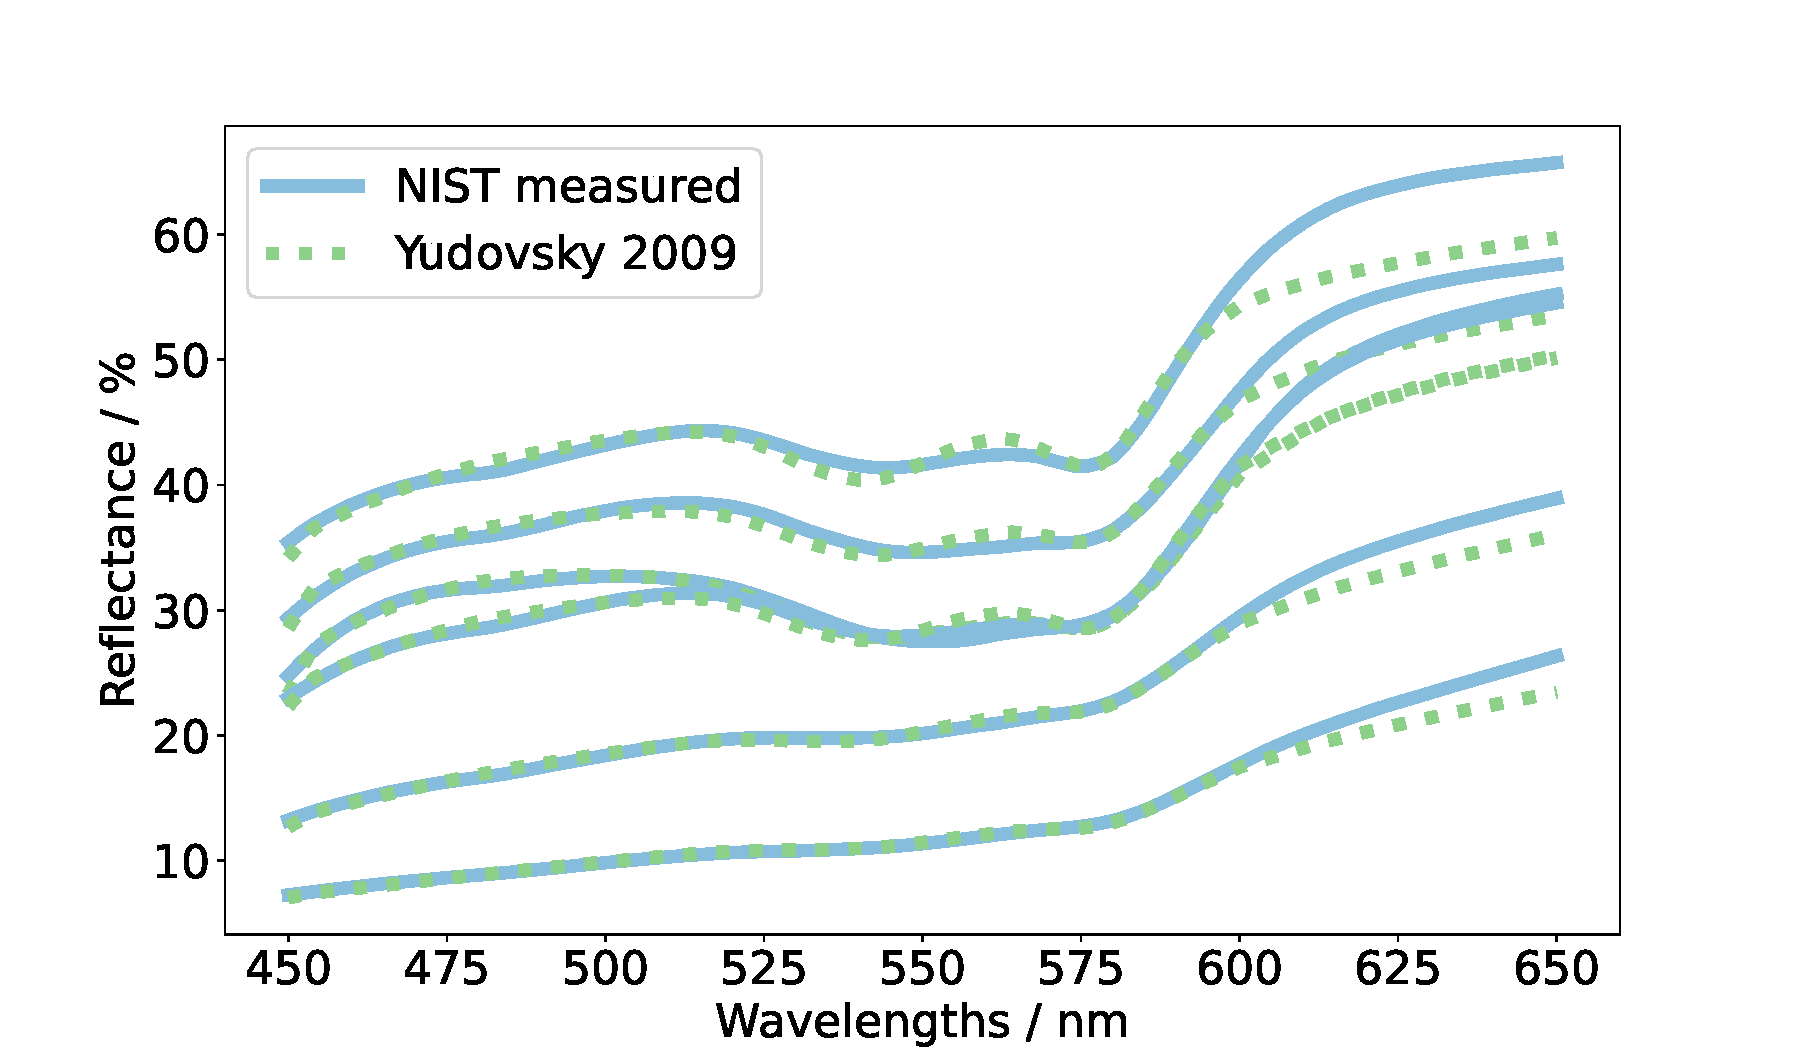
\includegraphics[width=\textwidth]{NIST_Eg_uniform.pdf}
        \caption{Quantitative}
        \label{fig:egspectraNISTu}
    \end{subfigure}
    \begin{subfigure}{0.49\textwidth}
        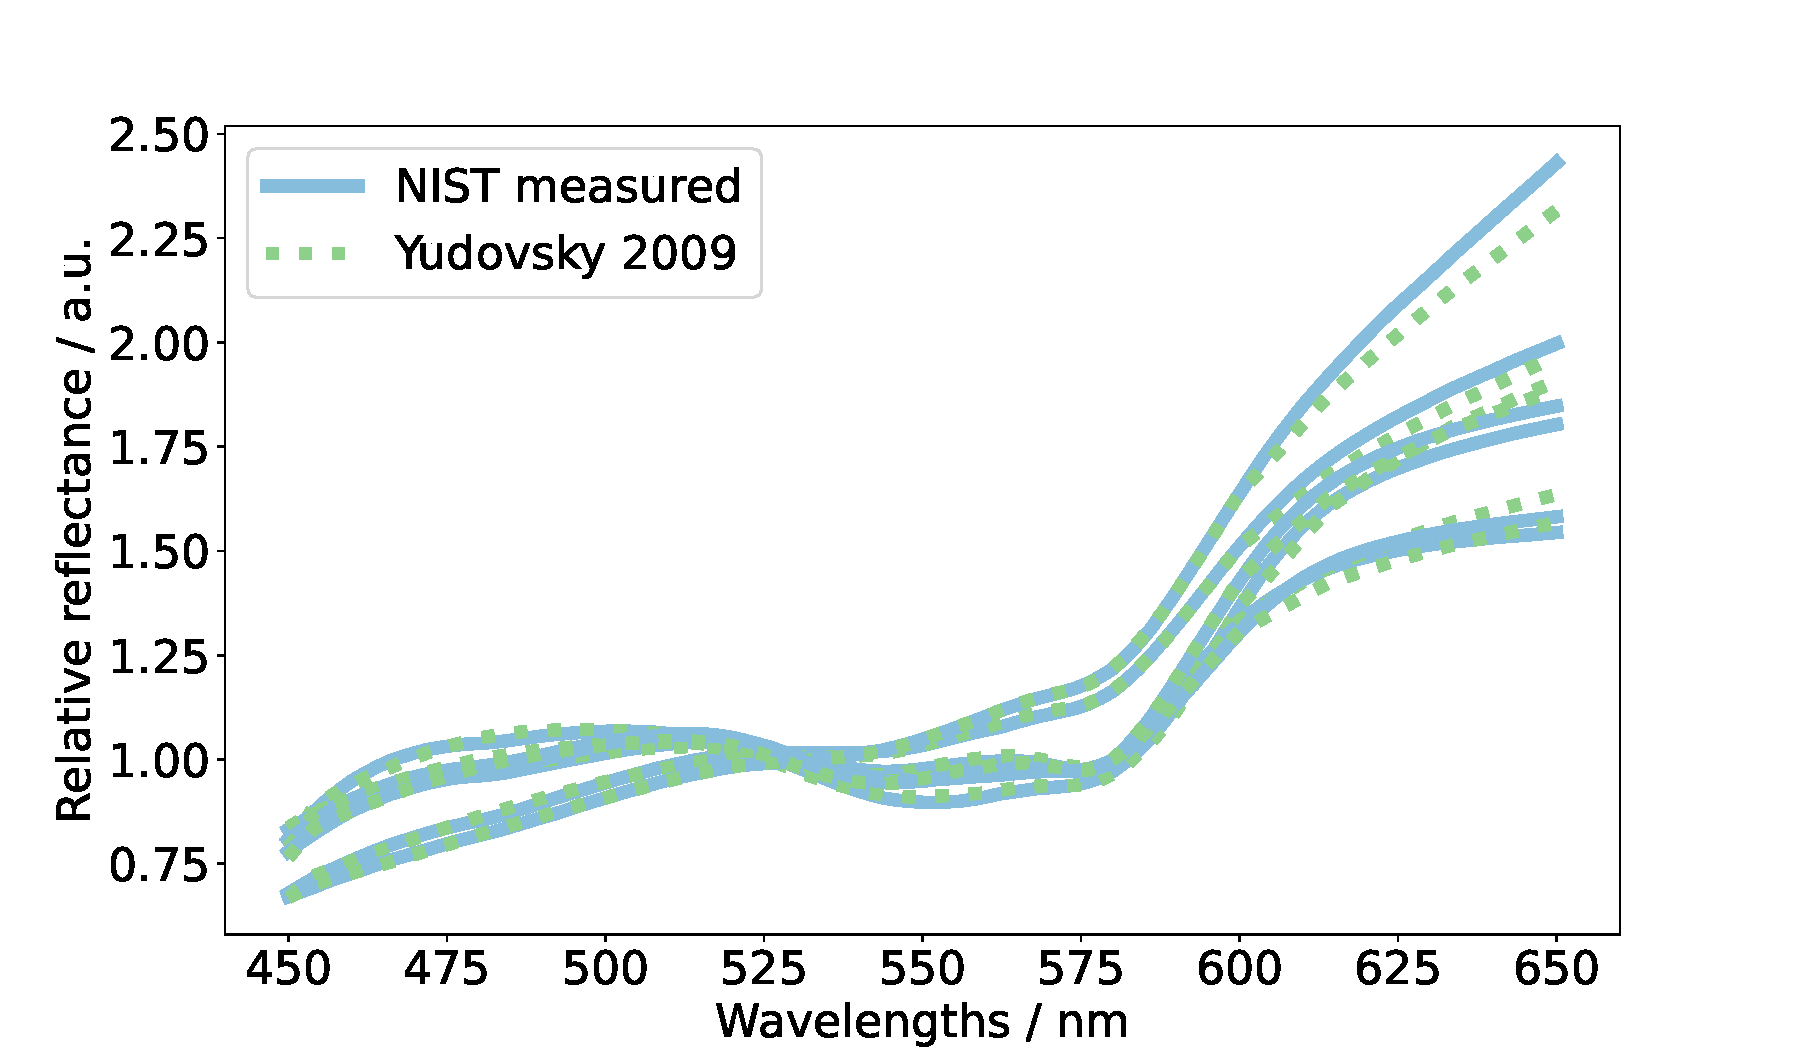
\includegraphics[width=\textwidth]{NIST_Eg_norm_uniform.pdf}
        \caption{Relative}
        \label{fig:egspectraNISTnormu}
    \end{subfigure}
    \begin{subfigure}{0.49\textwidth}
        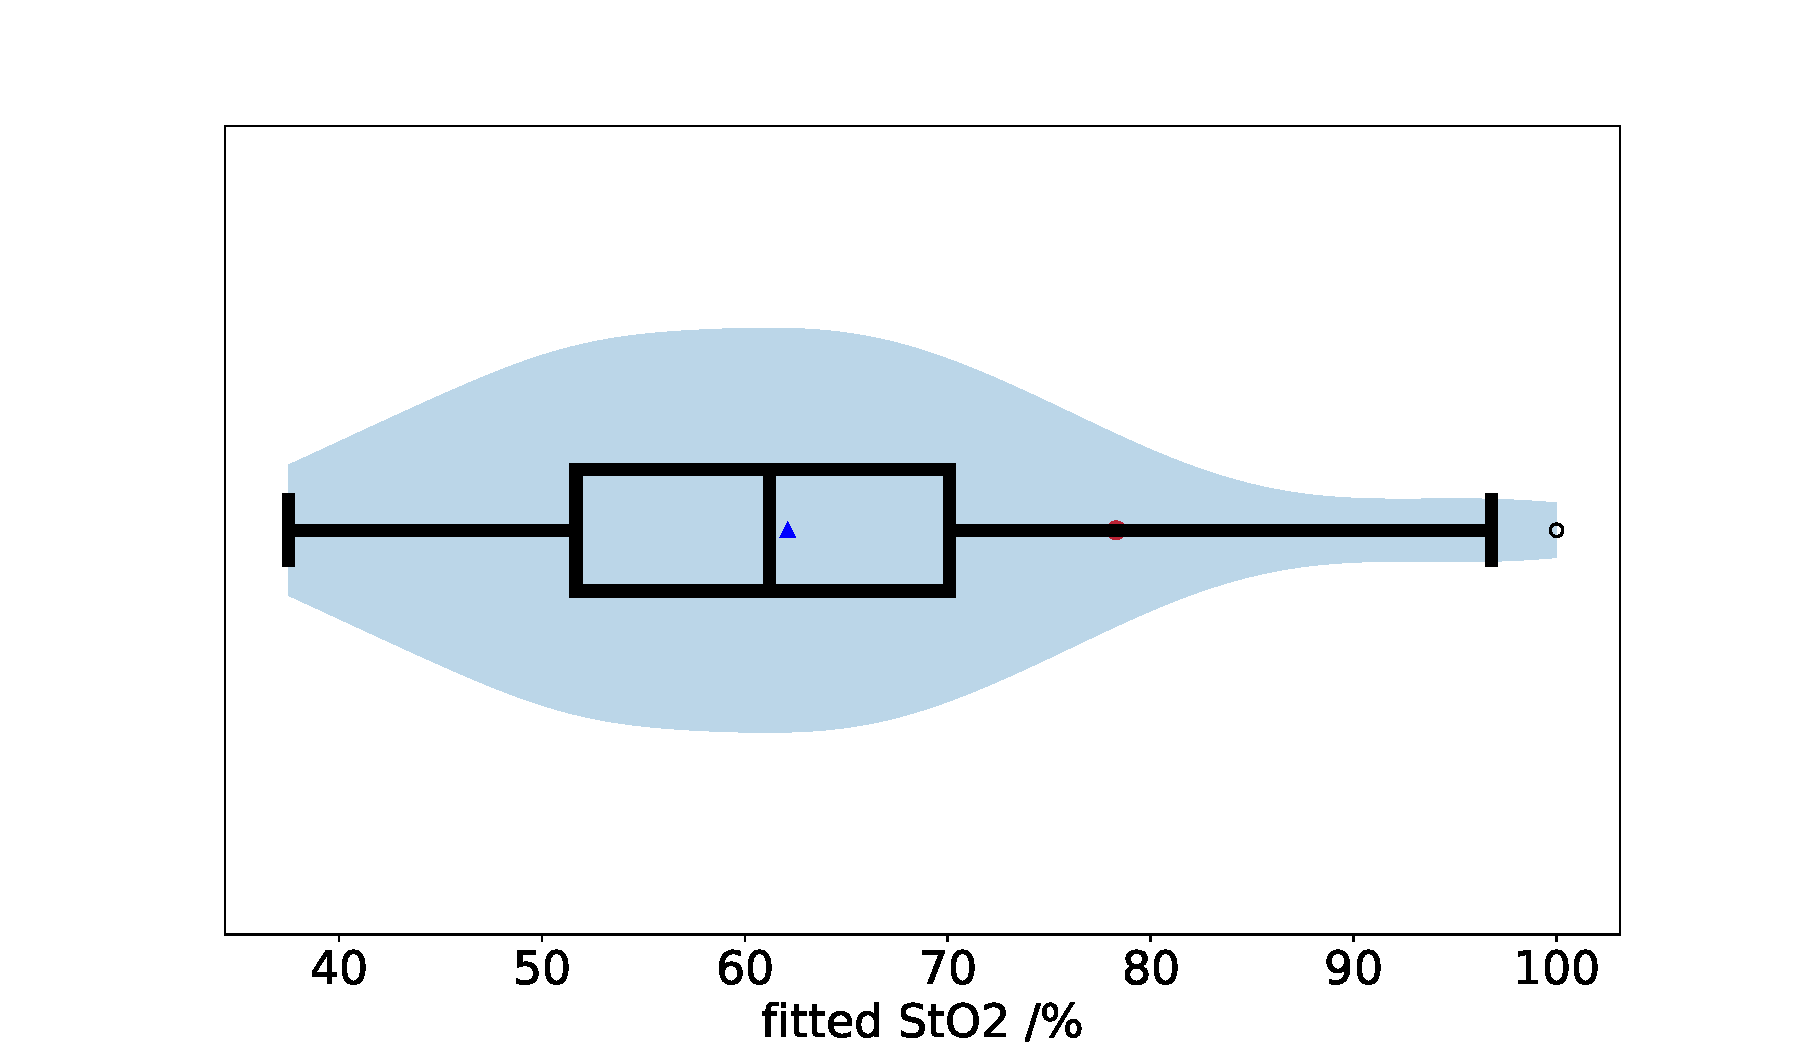
\includegraphics[width=\textwidth]{StO2_boxplot_uniform.pdf}
        \caption{Quantitative}
        \label{fig:egparamStO2NISTu}
    \end{subfigure}
    \begin{subfigure}{0.49\textwidth}
        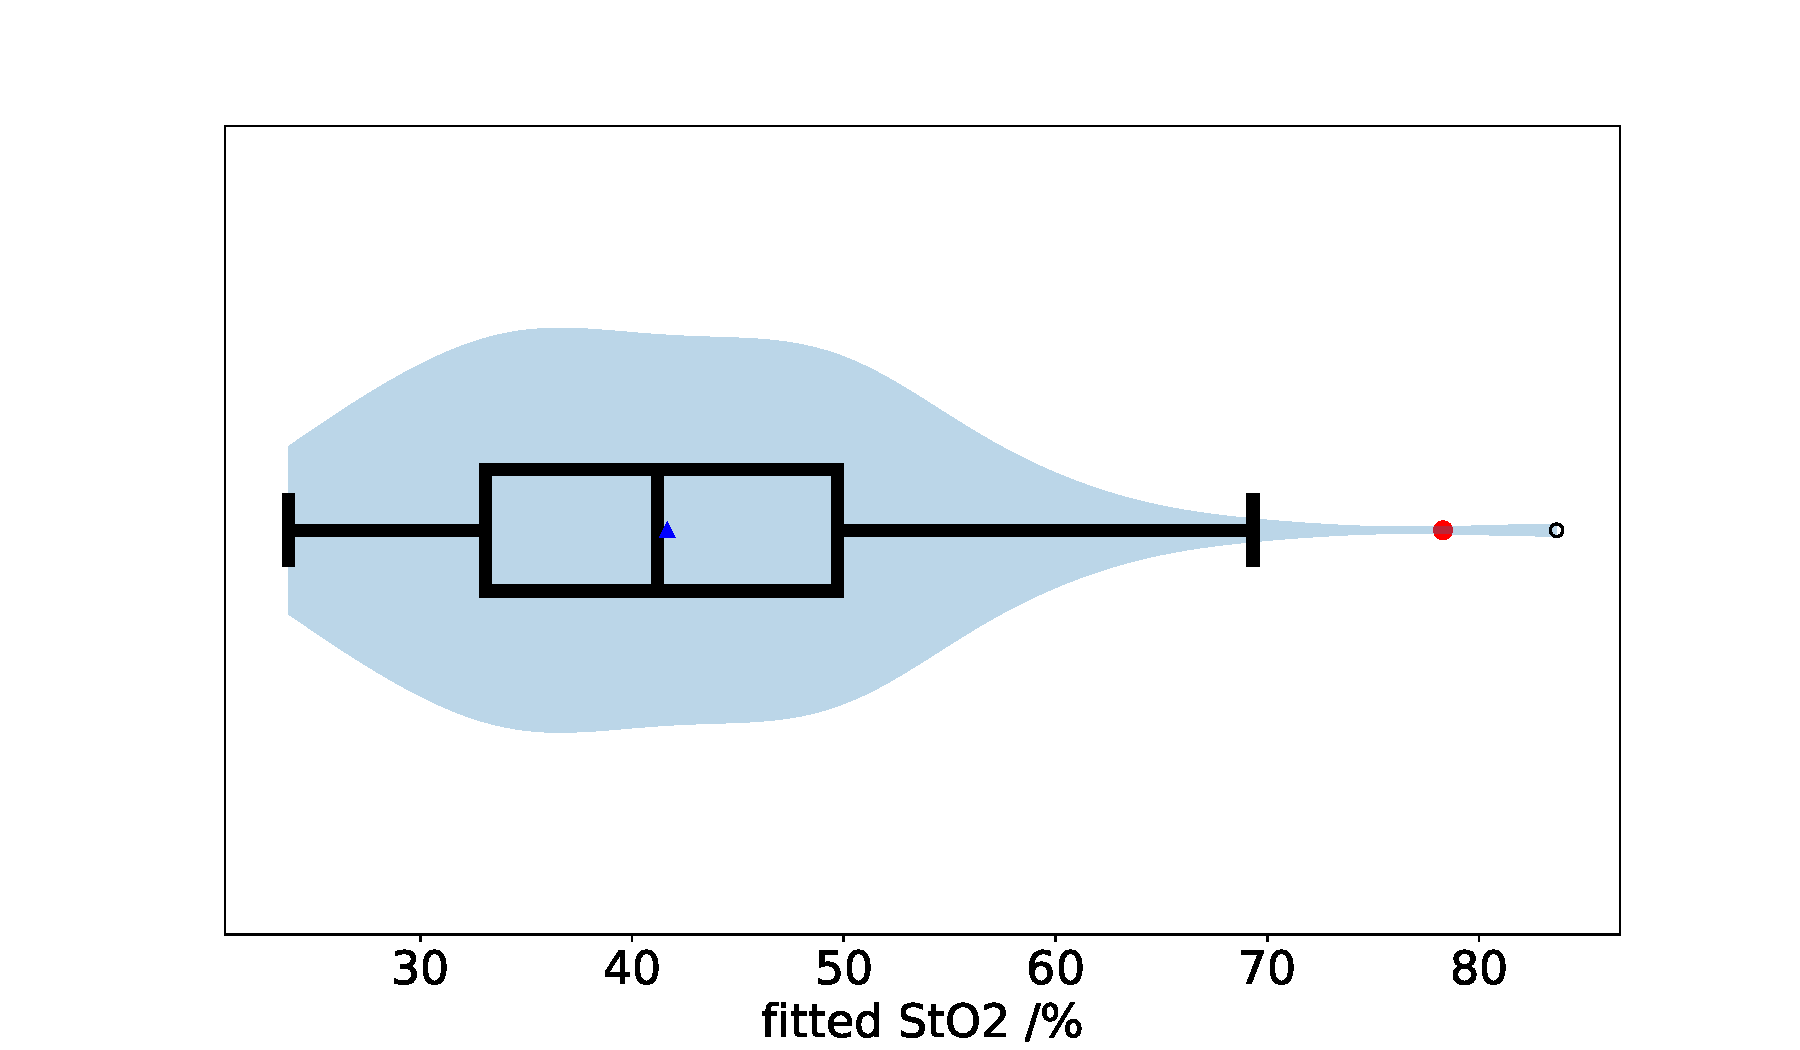
\includegraphics[width=\textwidth]{StO2_boxplot_norm_uniform.pdf}
        \caption{Relative}
        \label{fig:egparamStO2NISTnormu}
    \end{subfigure}
    \caption{Top: Examples of the Yudovsky 2009 two layer model fitted to NIST skin total reflectance spectra (\figref{fig:egspectraNIST}) for quantitative (left) or relative (right) data. Bottom: Box and violin plots displaying the retrieved $StO_2$ parameters from fitting the Yudovsky 2009 two layer model to the mean NIST skin spectra, where the triangle shows the mean of the fitted $StO_2$ and the circle shows a literature healthy dermis $StO_2$ value \citep{VanManen2021} for quantitative (left) or relative (right) data.}
    \label{fig:NISTuniform}
\end{figure}
\begin{table}[h]
    \centering
    \caption{The mean and standard deviation for each variable when extracted by fitting Yudovsky 2009 two layer model to the quantitative (Q) or relative (R) NIST skin reflectance dataset, compared to literature parameters for healthy individuals. All presented to 3s.f.}
    \begin{tabular}{|c|ccc|ccc|}
        \hline
         & \multicolumn{3}{c}{Extracted from NIST dataset} & \multicolumn{3}{|c|}{Literature} \\
        \cline{2-7}
         \rot{Parameter} & Q or R & \multirow{2}{*}{Mean} & Standard & \multirow{2}{*}{Mean} & Standard & \multirow{2}{*}{Source} \\
         & &  & deviation &  & deviation &  \\
        \hline
        $StO_2$ & Q & 62.1 & 14.5 & \multirow{2}{*}{78.3, 71} & \multirow{2}{*}{12.9, 16} & \cite{VanManen2021}, \\ %van manen http://dx.doi.org/10.21037/qims-21-46
        (\%) & R & 41.7 & 11.0 & & & \cite{Nishidate2011} \\ %Noninvasive imaging of human skin hemodynamicsusing a digital red-green-blue camera
        \hline
        $f_{blood}$ & Q & 0.875 & 0.443 & \multirow{2}{*}{1.1} & \multirow{2}{*}{0.4} & \multirow{2}{*}{\cite{Nishidate2011}} \\ %Noninvasive imaging of human skin hemodynamicsusing a digital red-green-blue camera
        (\%) & R & 1.66 & 0.996 & & & \\
        \hline
        $f_{mel}$ & Q & 2.57 & 3.95 & \multirow{2}{*}{4.3} & \multirow{2}{*}{1.2} & \multirow{2}{*}{\cite{Nishidate2011}} \\ %Noninvasive imaging of human skin hemodynamicsusing a digital red-green-blue camera
        (\%) & R & 3.03 & 2.18 & & &  \\
        \hline
        $L_1$ & Q & 66.2 & 20.5 & \multirow{2}{*}{75.5} & \multirow{2}{*}{N/A} & \multirow{2}{*}{\cite{Lintzeri2022}} \\ %https://www.webofscience.com/wos/woscc/full-record/WOS:000782026000001
        ($\mu$m) & R & 147 & 8.74 & & &  \\
        \hline
        $a$ & Q & 70.0 & 2.29$\times 10^{-8}$ & \multirow{2}{*}{46.0} & \multirow{2}{*}{13.7} & \multirow{2}{*}{\cite{Jacques2013}} \\ %Jacques review
        (\textrm{$cm^{-1}$}) & R & 45.7 & 11.4 & & &  \\
        \hline
        $b$ & Q & 1.01 & 0.382 & \multirow{2}{*}{1.421} & \multirow{2}{*}{0.517} & \multirow{2}{*}{\cite{Jacques2013}} \\ %Jacques review
        (a.u.) & R & 2.46 & 0.221 & & &  \\
        \hline
    \end{tabular}
    \label{tb:NISTparamsuniform}
\end{table}
\end{subappendices}